%%%%%%%%%%%%%%%%%%%%%%%%%%%%%%%%%%%%%%%%%
% Master Thesis Defense -- Alejandro Treny Ortega
% Measuring the Shape of Science
%
% Built on the LaTeXTemplates Beamer Presentation template v2.0
% (https://www.LaTeXTemplates.com, author Vel, CC BY-NC-SA 4.0),
% keeping its Madrid theme and structure. Evidence figures are the
% original vector figures from the thesis manuscript.
%%%%%%%%%%%%%%%%%%%%%%%%%%%%%%%%%%%%%%%%%

%----------------------------------------------------------------------------------------
%	PACKAGES AND OTHER DOCUMENT CONFIGURATIONS
%----------------------------------------------------------------------------------------

\documentclass[
	11pt, % Default font size
	aspectratio=169, % 16:9 aspect ratio to match modern screens and projectors
]{beamer}

\graphicspath{{assets/}{Images/}{./}} % Where to look for included images

\usepackage{booktabs} % Allows the use of \toprule, \midrule and \bottomrule for better rules in tables
\usepackage{amsmath} % Mathematical typesetting

%----------------------------------------------------------------------------------------
%	SELECT LAYOUT THEME
%----------------------------------------------------------------------------------------

\usetheme{Madrid}

%----------------------------------------------------------------------------------------
%	SELECT COLOR THEME
%----------------------------------------------------------------------------------------

% UC3M corporate blue (same azulUC3M used on the thesis cover), applied to the
% Madrid layout as the structure color.
\definecolor{UC3MBlue}{RGB}{0,0,102}
\usecolortheme[named=UC3MBlue]{structure}

%----------------------------------------------------------------------------------------
%	SELECT FONT THEME & FONTS
%----------------------------------------------------------------------------------------

\usefonttheme{default} % Typeset using the default sans serif font
\usepackage{palatino} % Use the Palatino font for serif text
\usepackage[default]{opensans} % Use the Open Sans font for sans serif text

%----------------------------------------------------------------------------------------
%	SELECT INNER THEME
%----------------------------------------------------------------------------------------

\useinnertheme{circles}

%----------------------------------------------------------------------------------------
%	GLOBAL ADJUSTMENTS
%----------------------------------------------------------------------------------------

\setbeamertemplate{navigation symbols}{} % Remove the navigation symbols from the bottom of all slides

% Keep the frame count shown in the footline equal to the last numbered slide of
% the main deck, so backup slides do not inflate the total.
\newcommand{\backupbegin}{
	\newcounter{finalframe}
	\setcounter{finalframe}{\value{framenumber}}
}
\newcommand{\backupend}{
	\setcounter{framenumber}{\value{finalframe}}
}

% Small gray note line used under evidence figures.
\newcommand{\fignote}[1]{{\par\vspace{2pt}\footnotesize\textcolor{gray}{#1}\par}}

%----------------------------------------------------------------------------------------
%	PRESENTATION INFORMATION
%----------------------------------------------------------------------------------------

\title[Measuring the Shape of Science]{Measuring the Shape of Science}

\subtitle{Morphological Indicators and Evolution of Research Fields}

\author[A. Treny Ortega]{Alejandro Treny Ortega \\ \smallskip {\small Supervisor: Mar\'ia Luz Durb\'an Reguera}}

\institute[UC3M]{Master in Statistics for Data Science \\ Universidad Carlos III de Madrid}

\date[July 2026]{Master Thesis Defense \\ July 2026}

\titlegraphic{
\includegraphics[width=0.30\textwidth]{logo_UC3M.png}}

%----------------------------------------------------------------------------------------

\begin{document}

%----------------------------------------------------------------------------------------
%	TITLE SLIDE
%----------------------------------------------------------------------------------------

\begin{frame}
	\titlepage
\end{frame}

%----------------------------------------------------------------------------------------
%	TABLE OF CONTENTS SLIDE
%----------------------------------------------------------------------------------------

\begin{frame}
	\frametitle{Outline}

	\tableofcontents
\end{frame}

%----------------------------------------------------------------------------------------
%	PRESENTATION BODY SLIDES
%----------------------------------------------------------------------------------------

\section{Problem and Measurement}

%------------------------------------------------

\begin{frame}
	\frametitle{A scientific field is a cloud of documents}

	A field label says what research is \emph{called}, not how its papers are \alert{arranged}.

	\begin{center}
		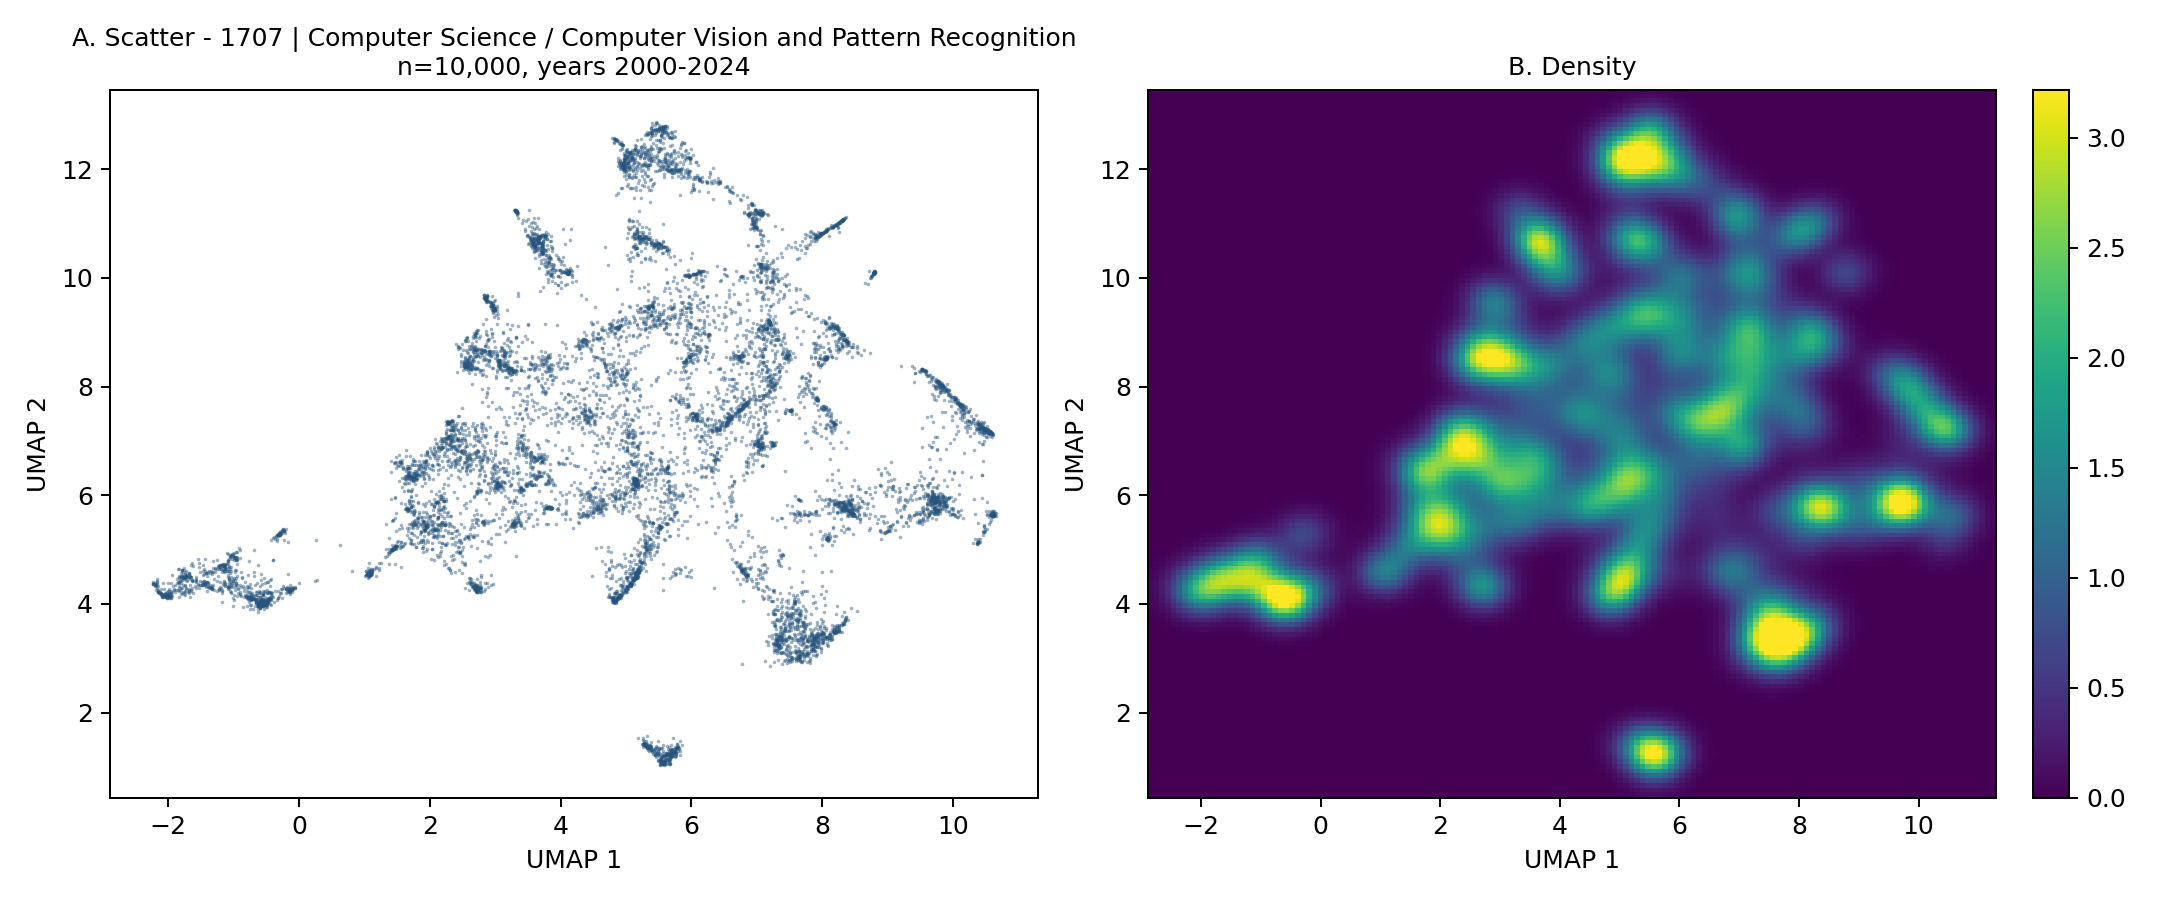
\includegraphics[width=0.71\linewidth]{fig_d_umap_computer_vision_pattern_recognition.png}
	\end{center}
	\fignote{One subfield, seen from above: 10{,}000 Computer Vision papers, placed by similarity of title and abstract.}

	\smallskip
	\textbf{Central idea:} treat each field as a \alert{cloud of papers} and measure the \alert{shape} of that cloud.
\end{frame}

%------------------------------------------------

\begin{frame}
	\frametitle{Three questions about the shape of science}

	\begin{enumerate}
		\setlength{\itemsep}{1.0em}
		\item Can we \alert{measure} the shape of a scientific field?
		\item Does that shape \alert{differ} across sciences, and does it \alert{change} over time?
		\item Which fields are \alert{moving closer together}, and which are \alert{drifting apart}?
	\end{enumerate}

	\bigskip

	\centering
	\textbf{25 years of science, 2.3 million papers, one measuring stick.}
\end{frame}

%------------------------------------------------

\begin{frame}
	\frametitle{A balanced OpenAlex corpus makes 241 subfields comparable}

	\begin{center}
		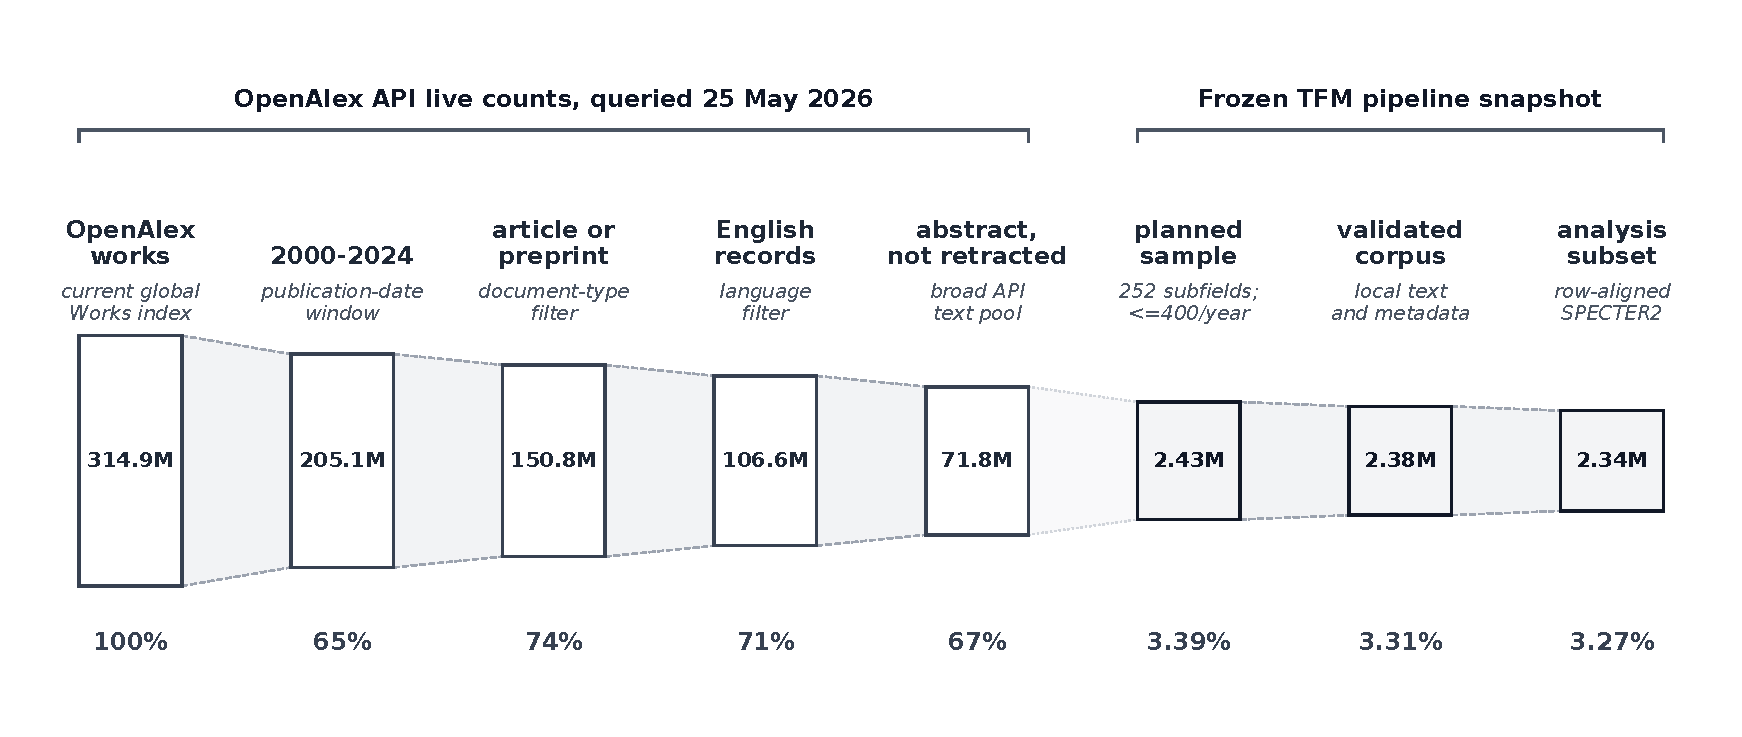
\includegraphics[width=0.88\linewidth]{fig_03_openalex_corpus_pipeline.pdf}
	\end{center}

	\smallskip
	\centering
	{\small \textbf{2{,}344{,}927} papers \;\textbullet\; \textbf{241} subfields \;\textbullet\; \textbf{26} fields \;\textbullet\; \textbf{4} domains\par}
	\smallskip
	{\footnotesize\textcolor{gray}{Subfields are the measuring unit; a field's shape is the average of its subfields.\\
	Same yearly cap for every subfield: fields are compared on shape, not on publication volume.}\par}
\end{frame}

%------------------------------------------------

\begin{frame}
	\frametitle{Every paper becomes a point in the same space}

	\begin{itemize}
		\setlength{\itemsep}{0.9em}
		\item SPECTER2, a language model trained on scientific papers, reads each title and abstract and turns it into \textbf{768 numbers}: a point in space.
		\item Papers about similar research land \alert{close together}; unrelated research lands far apart.
		\item A field is then a cloud of points, and the shape of that cloud \alert{can be measured}.
	\end{itemize}

	\bigskip

	\begin{block}{One rule, applied everywhere}
		Every number in this thesis is computed in the full 768-dimensional space. Maps like the previous one are only for looking.
	\end{block}
\end{frame}

%------------------------------------------------

\begin{frame}
	\frametitle{Eight numbers describe the shape of a field}

	\begin{table}
		\centering
		\footnotesize
		\begin{tabular}{@{}l l p{5.5cm}@{}}
			\toprule
			\textbf{Family} & \textbf{Metrics} & \textbf{Question answered} \\
			\midrule
			Spread & Centroid median, IQR, P90 & How far do papers spread out? \\
			Local packing & kNN median, kNN CV & How tightly are neighbours packed? \\
			Hubs & kNN in-degree Gini & Do a few papers dominate? \\
			Dimensionality & PCA $D_{80}$, PCA entropy & How many directions are needed? \\
			\bottomrule
		\end{tabular}
	\end{table}

	\bigskip

	\begin{block}{Eight numbers, kept separate}
		Each family captures a different kind of shape: a field can be broad but tightly packed, or compact but dominated by a few hub papers.
	\end{block}
\end{frame}

%------------------------------------------------

\begin{frame}
	\frametitle{Spread: how far papers reach from the field centre}

	\begin{center}
		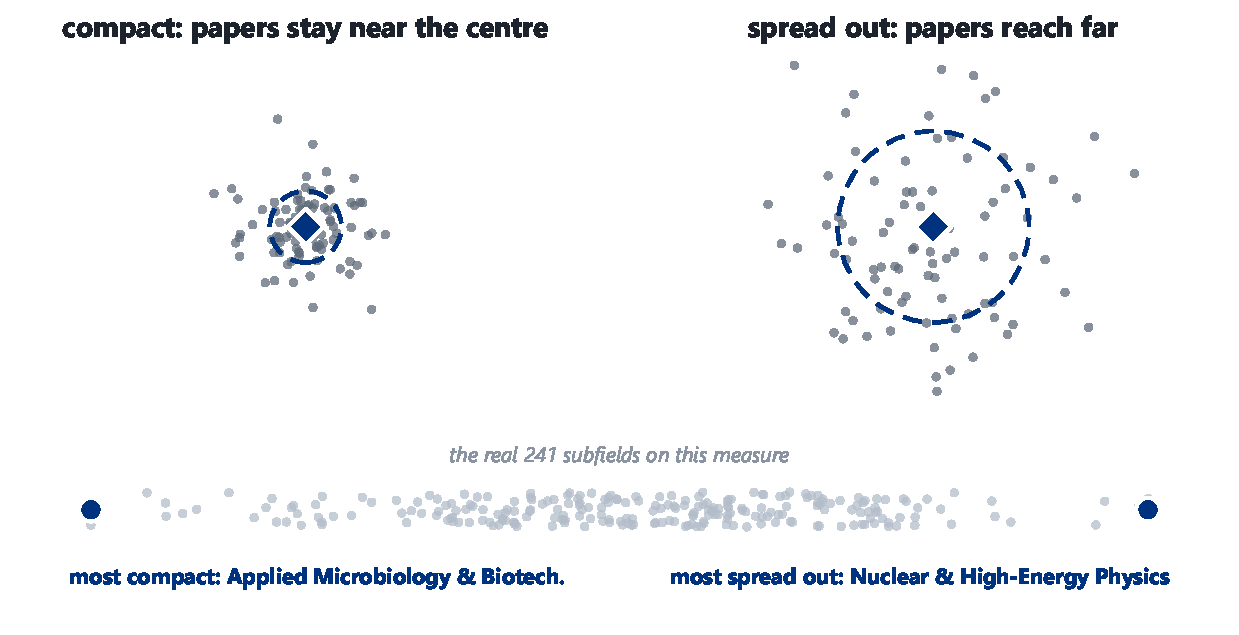
\includegraphics[height=0.84\textheight]{def_family_spread.pdf}
	\end{center}
\end{frame}

%------------------------------------------------

\begin{frame}
	\frametitle{Local packing: how close neighbouring papers sit}

	\begin{center}
		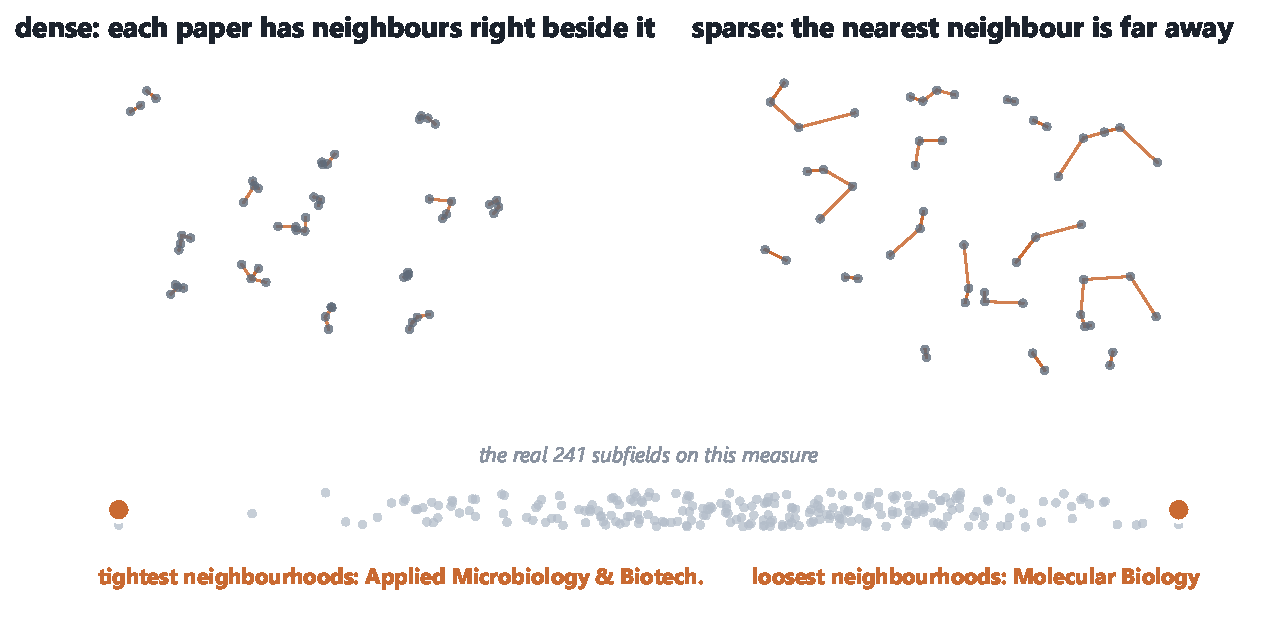
\includegraphics[height=0.84\textheight]{def_family_packing.pdf}
	\end{center}
\end{frame}

%------------------------------------------------

\begin{frame}
	\frametitle{Hubs: whether a few papers dominate}

	\begin{center}
		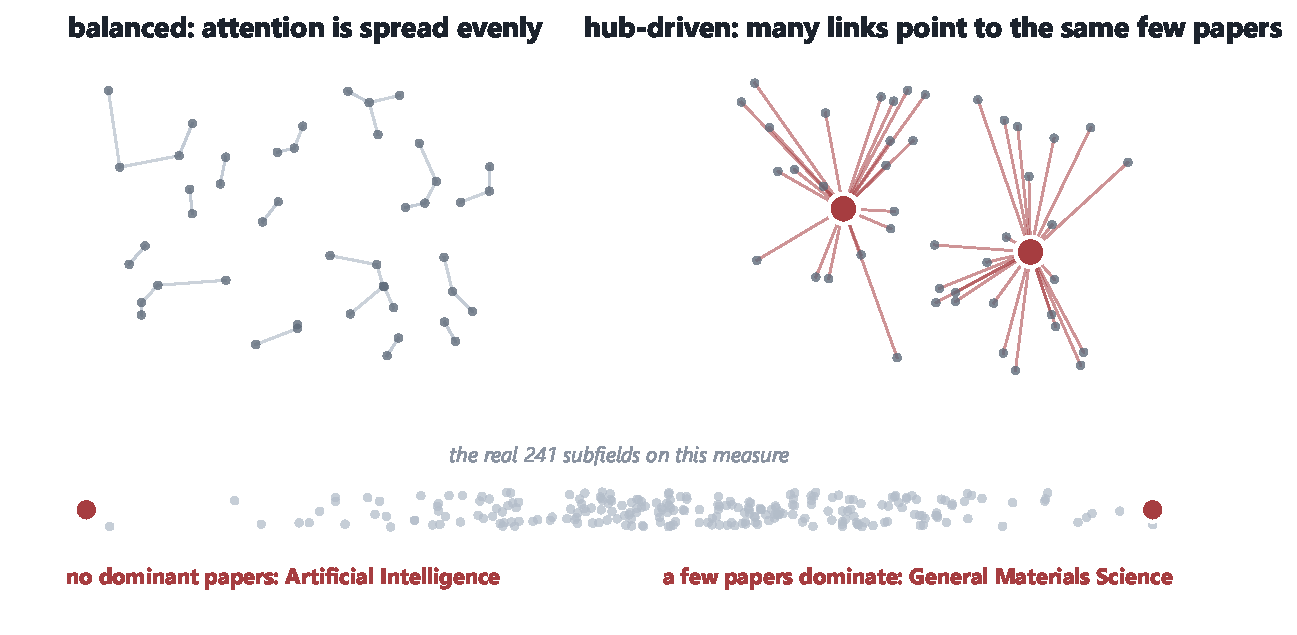
\includegraphics[height=0.84\textheight]{def_family_hubs.pdf}
	\end{center}
\end{frame}

%------------------------------------------------

\begin{frame}
	\frametitle{Dimensionality: how many directions the variation needs}

	\begin{center}
		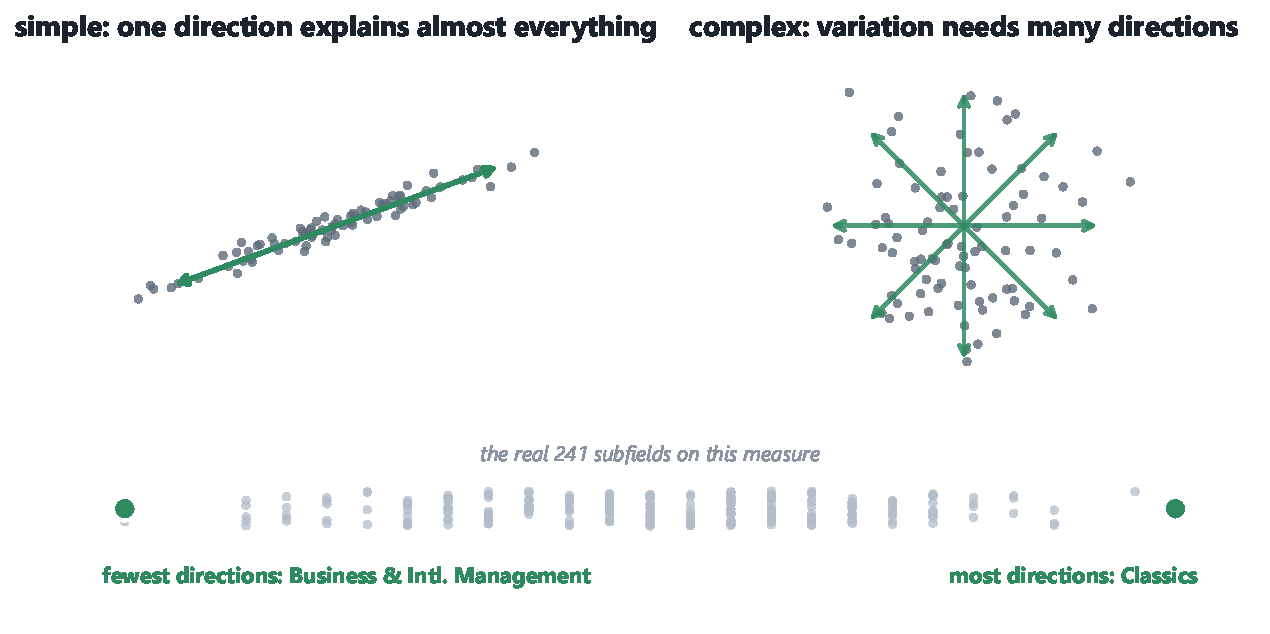
\includegraphics[height=0.84\textheight]{def_family_dims.pdf}
	\end{center}
\end{frame}

%------------------------------------------------

\section{Static Morphology of Fields}

%------------------------------------------------

\begin{frame}
	\frametitle{The loosest and tightest corners of science}

	\begin{center}
		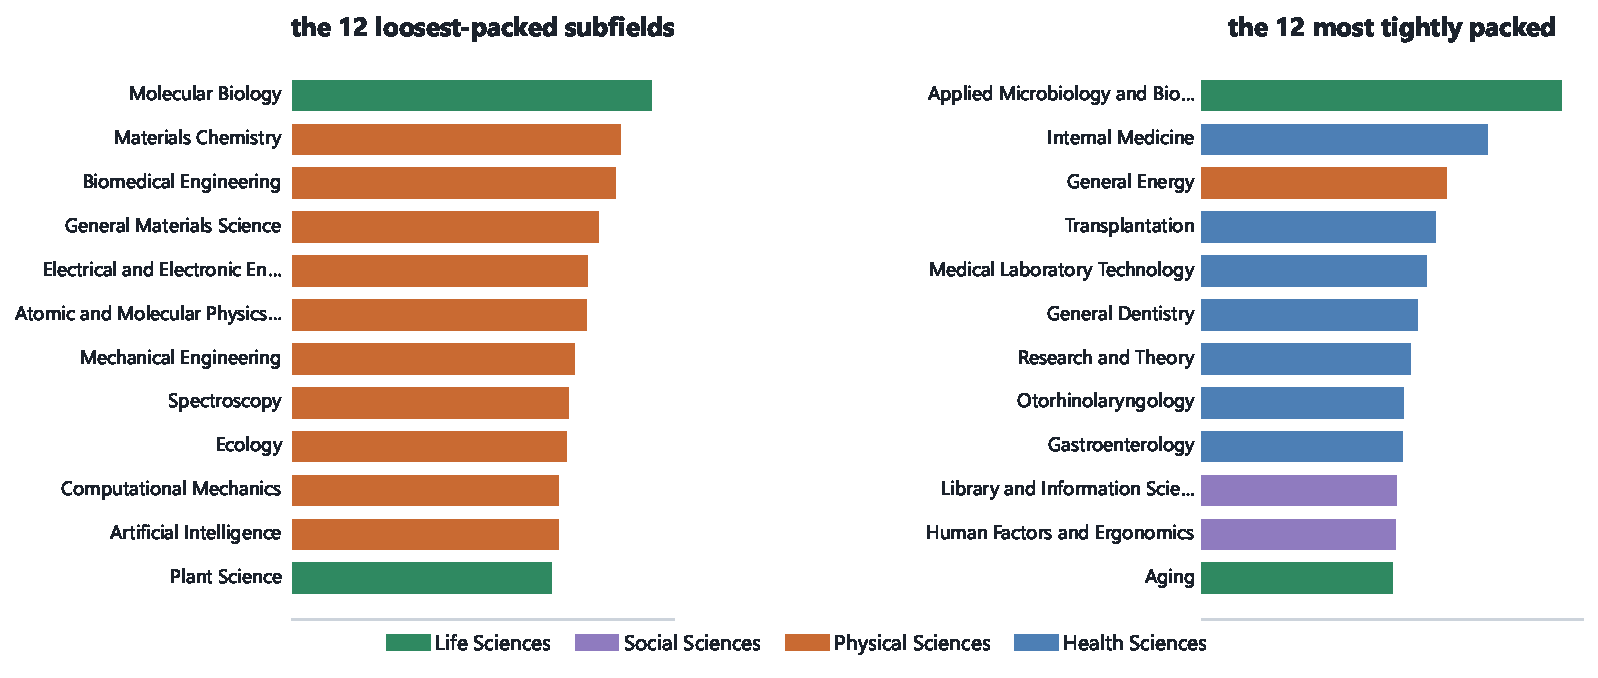
\includegraphics[width=0.92\linewidth]{def_opt_leaderboard.pdf}
	\end{center}

	\smallskip
	\centering
	The loose end is Physical Sciences territory; the tight end belongs to medicine and health.
\end{frame}

%------------------------------------------------

\begin{frame}
	\frametitle{The most similar shapes ignore domain borders}

	\begin{center}
		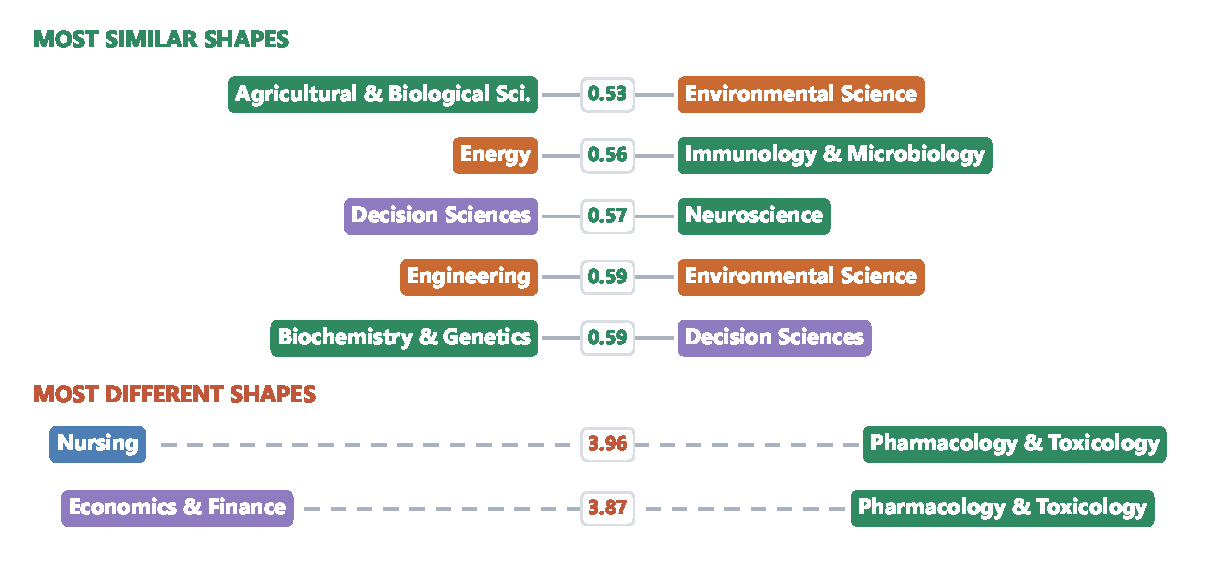
\includegraphics[height=0.74\textheight]{def_alike_pairs.pdf}
	\end{center}

	\smallskip
	\centering
	\textbf{7 of the 10} closest pairs join fields from \alert{different domains}.
\end{frame}

%------------------------------------------------

\section{Temporal Evolution}

%------------------------------------------------

\begin{frame}
	\frametitle{Science is packing tighter}

	\begin{center}
		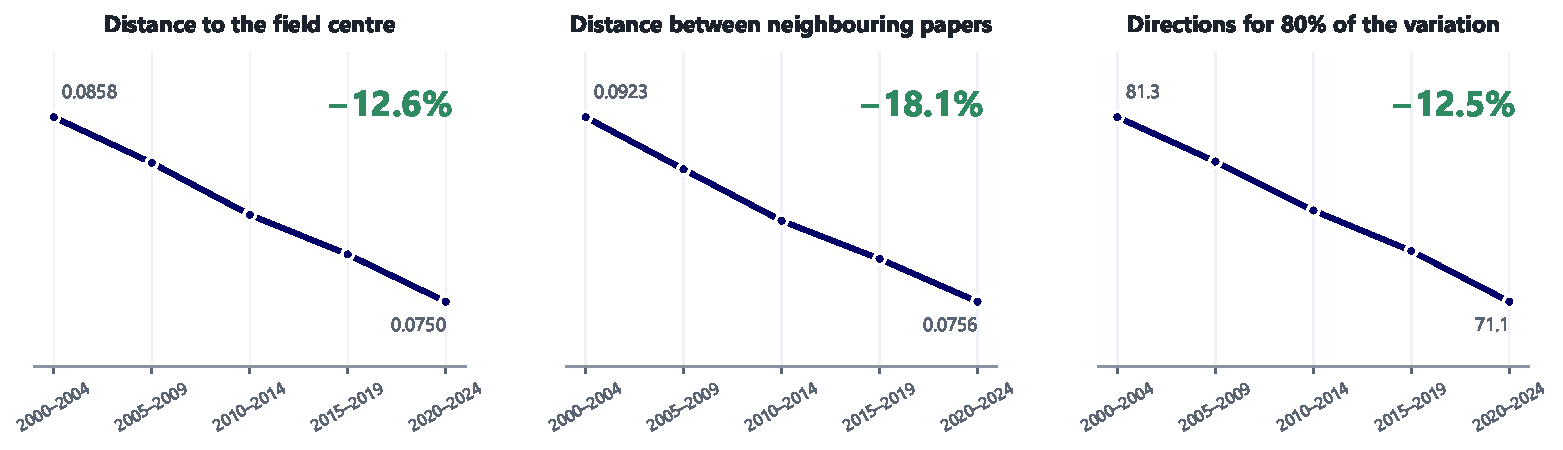
\includegraphics[width=0.95\linewidth]{def_packing_curves.pdf}
	\end{center}

	\medskip
	\centering
	Papers sit closer to their field's centre, closer to their neighbours, and vary along fewer directions.\\
	\smallskip
	And the tightening is \alert{uneven}: some neighbourhoods shrink much faster than others.
\end{frame}

%------------------------------------------------

\begin{frame}
	\frametitle{Changing shape is not the same as moving}

	\begin{columns}[c]
		\begin{column}{0.58\textwidth}
			\centering
			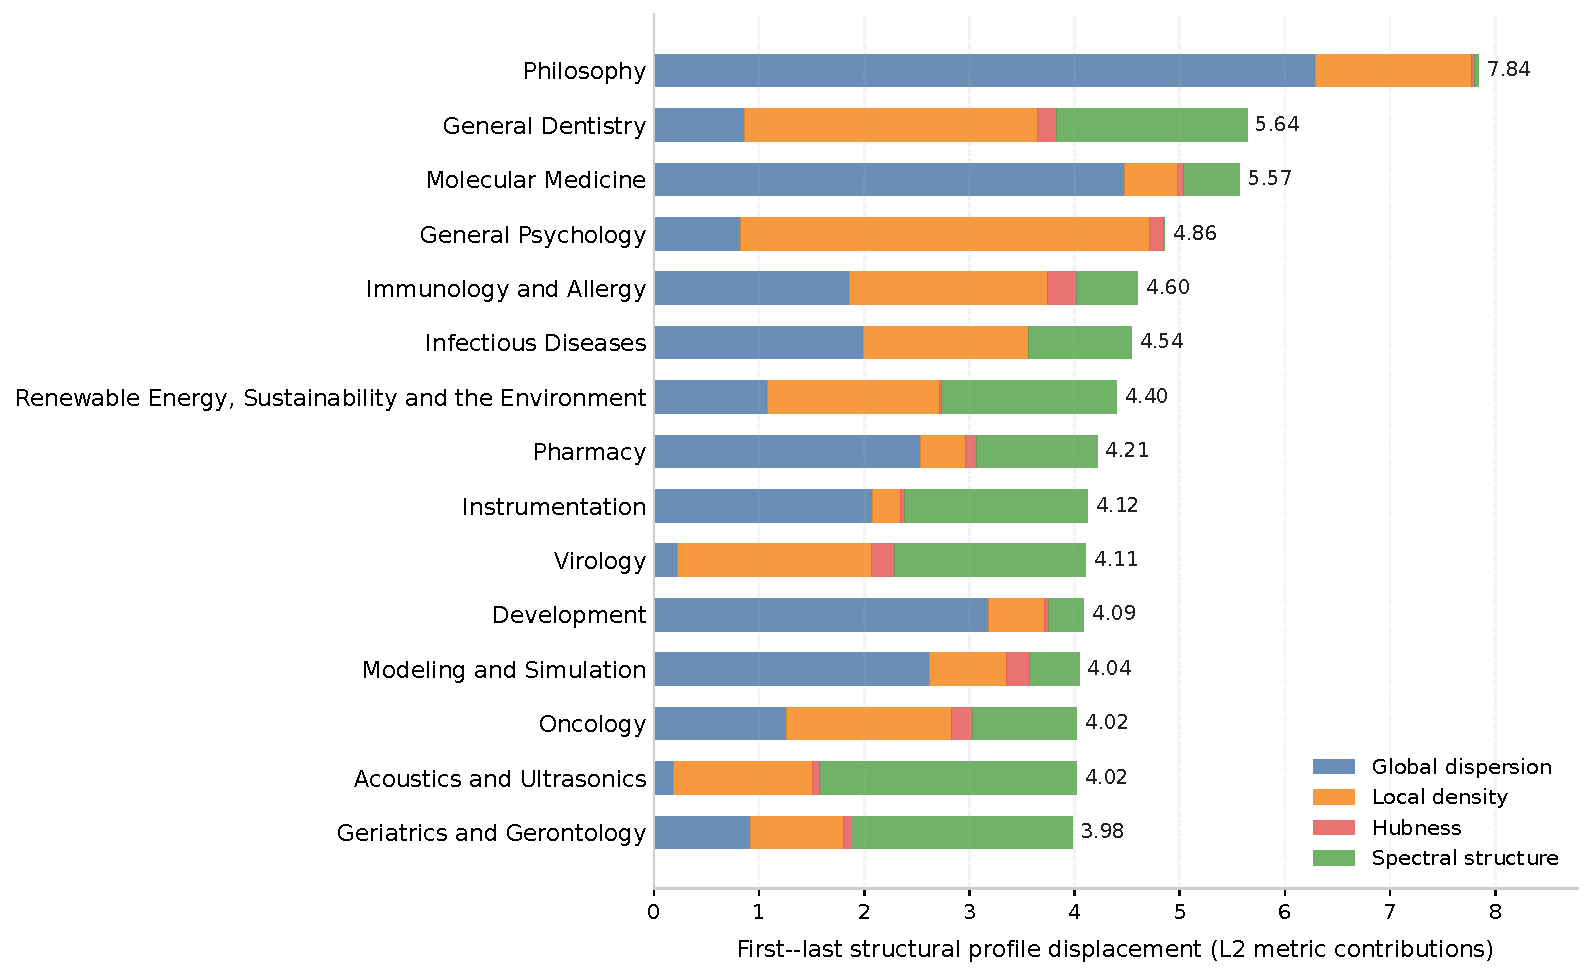
\includegraphics[width=\linewidth]{fig_05_most_dynamic_subfields.pdf}
		\end{column}
		\begin{column}{0.40\textwidth}
			\small
			\begin{block}{Biggest change in shape}
				\textbf{Philosophy}: its papers now spread far more \emph{evenly} around the centre than in 2000.
			\end{block}

			\medskip
			The colours show which shape family drives each change: a different mix for every subfield.
		\end{column}
	\end{columns}
\end{frame}

%------------------------------------------------

\begin{frame}
	\frametitle{Some fields travel, others stay put}

	\begin{columns}[c]
		\begin{column}{0.57\textwidth}
			\centering
			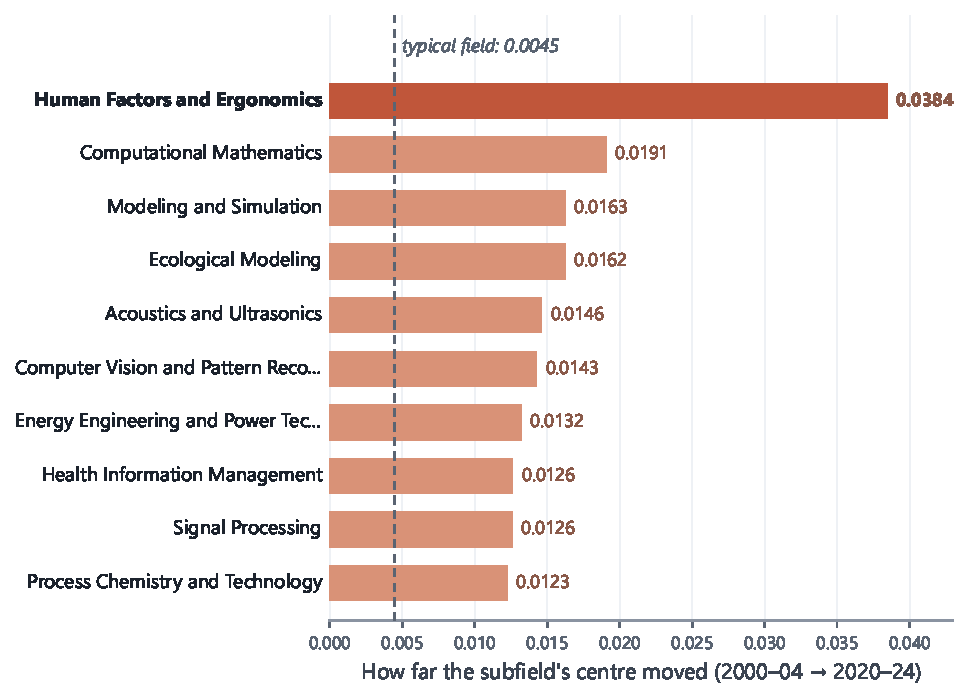
\includegraphics[width=\linewidth]{def_drift_movers.pdf}
		\end{column}
		\begin{column}{0.41\textwidth}
			\small
			\begin{block}{Biggest change of place}
				\textbf{Human Factors and Ergonomics}: its topics move $8.5\times$ further than the typical field.
			\end{block}

			\medskip
			The movers are applied, technology-driven areas. Mature theory (Mathematical Physics, Algebra, Geometry) barely moves in 25 years.

			\medskip
			A field can rebuild itself without moving, or move without rebuilding.
		\end{column}
	\end{columns}
\end{frame}

%------------------------------------------------

\section{Relations Between Fields}

%------------------------------------------------

\begin{frame}
	\frametitle{17 of 26 fields look most like a field from another domain}

	\begin{center}
		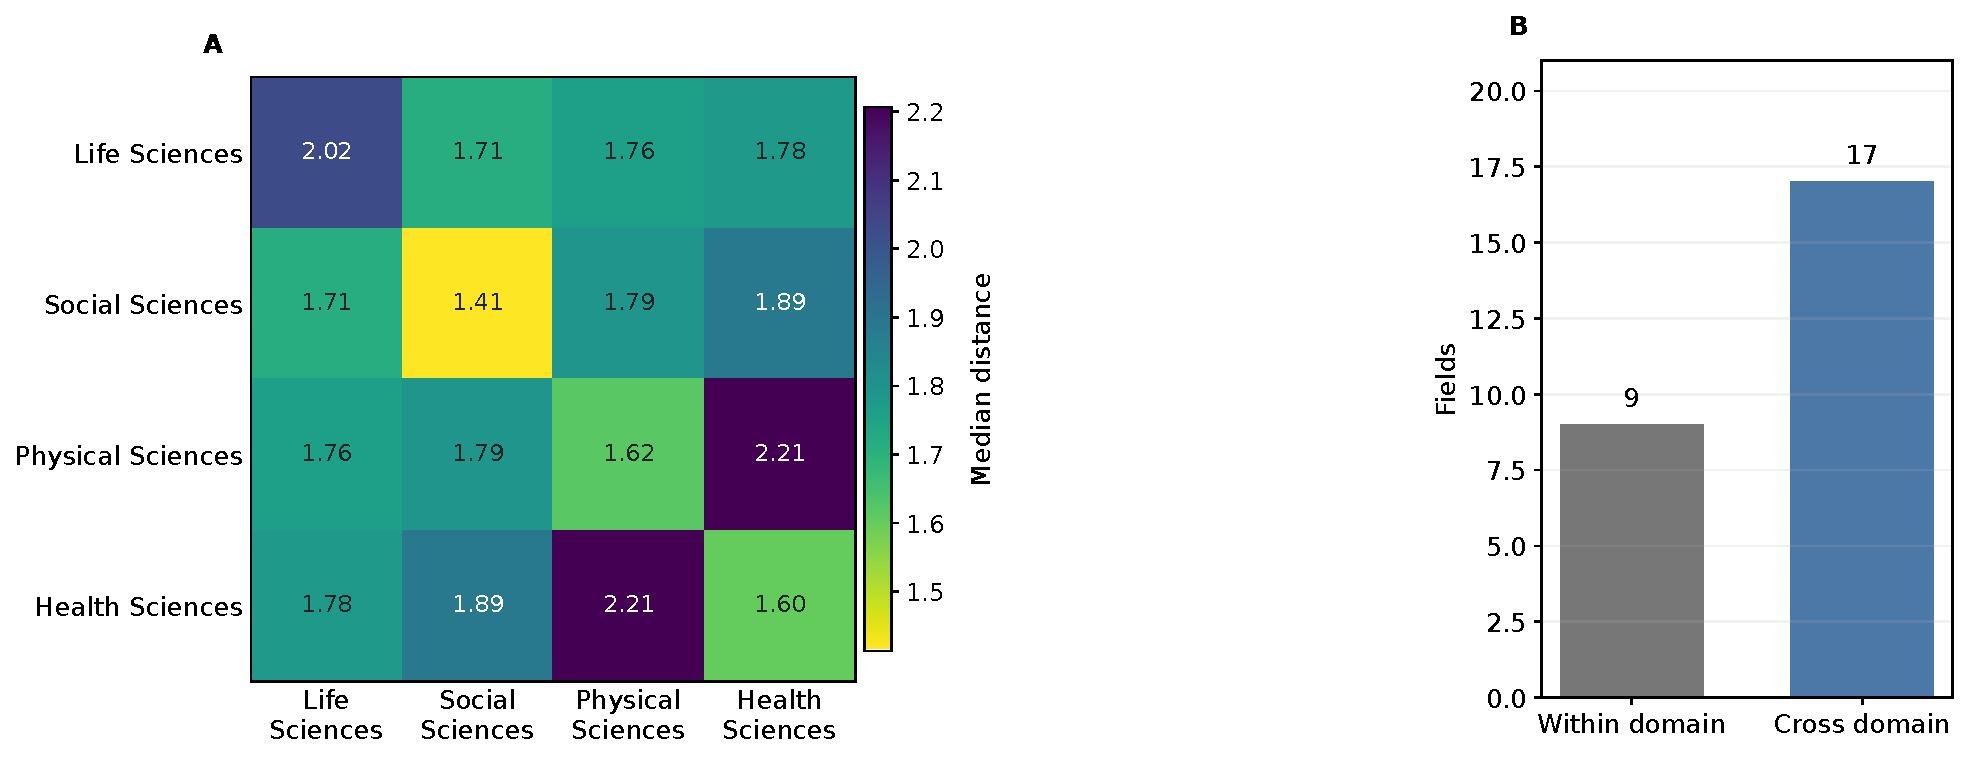
\includegraphics[width=0.93\linewidth]{fig_06_domain_pair_distance_structure.pdf}
	\end{center}

	\medskip
	\centering
	Fields from the same domain are somewhat closer in shape (\textbf{1.62} vs.\ \textbf{1.86}), yet for \textbf{65\%} of fields the most similar shape belongs to \alert{another} domain.
\end{frame}

%------------------------------------------------

\begin{frame}
	\frametitle{Yet field shapes are drifting apart: $+$25.7\% in twenty years}

	\begin{columns}[c]
		\begin{column}{0.56\textwidth}
			\centering
			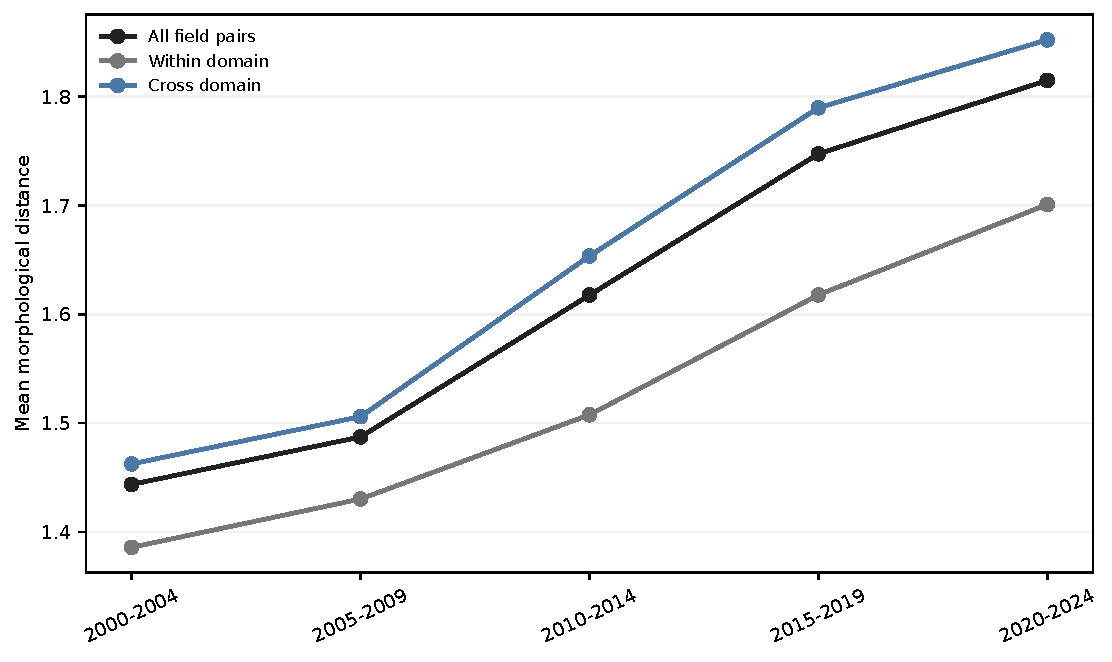
\includegraphics[width=\linewidth]{fig_06_temporal_distance_trajectories.pdf}
		\end{column}
		\begin{column}{0.42\textwidth}
			\begin{block}{Average distance between fields}
				\centering
				{\LARGE 1.44 $\rightarrow$ 1.81}\\
				\smallskip
				{\small from 2000--2004 to 2020--2024}
			\end{block}

			\medskip

			\begin{itemize}
				\setlength{\itemsep}{0.5em}
				\item \textbf{228} pairs of fields drift apart; only \textbf{97} move closer.
				\item The rise appears both inside domains and across them.
			\end{itemize}
		\end{column}
	\end{columns}
\end{frame}

%------------------------------------------------

\begin{frame}
	\frametitle{Computer Science is pulling away from everyone}

	\begin{center}
		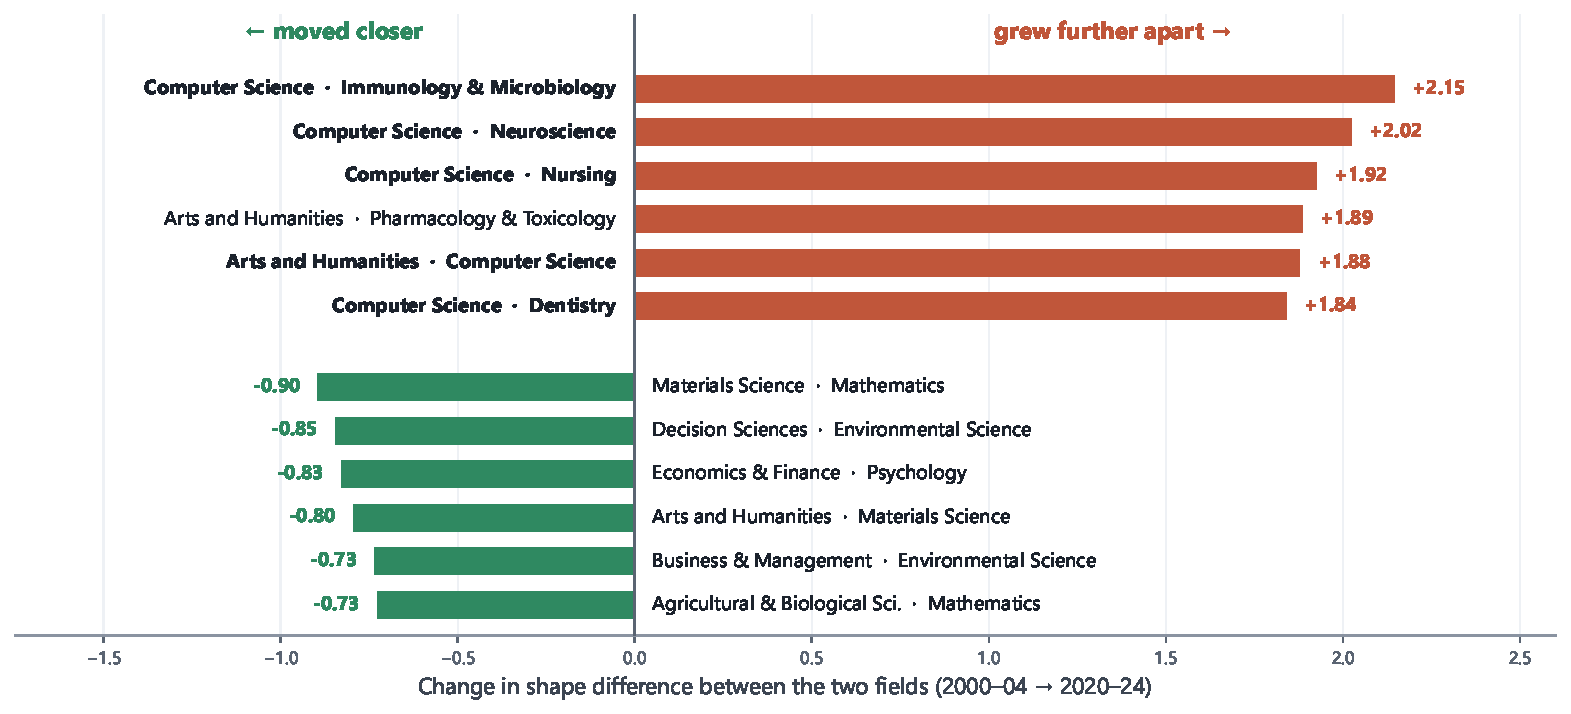
\includegraphics[height=0.66\textheight]{def_convergence.pdf}
	\end{center}

	\smallskip
	\centering
	Computer Science appears in \textbf{9 of the 10} biggest separations, while surprising couples such as Materials Science and Mathematics end up \textbf{50\% closer}.
\end{frame}

%------------------------------------------------

\section{Conclusions}

%------------------------------------------------

\begin{frame}
	\frametitle{Main findings}

	\begin{table}
		\centering
		\small
		\begin{tabular}{@{}ll@{}}
			\toprule
			\textbf{Finding} & \textbf{Evidence} \\
			\midrule
			Papers pack tighter inside their fields & Distance between neighbouring papers $-$18\% \\
			\addlinespace[0.65em]
			Research varies along fewer directions & From 81 to 71 main directions \\
			\addlinespace[0.65em]
			Field shapes drift apart & Average distance between fields $+$26\% \\
			\addlinespace[0.65em]
			Shape ignores the official map of science & 17 of 26 fields match a field from another domain \\
			\addlinespace[0.65em]
			Changing shape $\neq$ changing place & Philosophy reshapes; Human Factors moves \\
			\bottomrule
		\end{tabular}
	\end{table}

	\bigskip

	\centering
	\textbf{Science is packing tighter on the inside while its fields grow more different from each other.}
\end{frame}

%------------------------------------------------

\begin{frame}
	\frametitle{What this thesis contributes}

	\begin{itemize}
		\setlength{\itemsep}{0.9em}
		\item A \textbf{new, reproducible way to measure the shape} of a scientific field, comparable across all of science and across 25 years.
		\item One framework that answers three questions at once: what shape a field has, \textbf{how it changes}, and \textbf{which fields move together}.
		\item Everything is open: the code, the data pipeline, and an \textbf{interactive viewer} anyone can explore.
	\end{itemize}

	\bigskip

	\begin{block}{And a clear road ahead}
		The same measuring stick can be re-run with other language models, full text, or citation networks, so every finding can be stress-tested.
	\end{block}
\end{frame}

%----------------------------------------------------------------------------------------
%	CLOSING SLIDE
%----------------------------------------------------------------------------------------

\begin{frame}[plain]
	\begin{center}
		{\footnotesize\textcolor{gray}{MASTER THESIS DEFENSE \;\textbullet\; JULY 2026}}

		\vspace{0.65cm}

		{\LARGE\bfseries\textcolor{UC3MBlue}{Every field has a shape.}}

		\smallskip

		{\LARGE\bfseries\textcolor{UC3MBlue}{Now we can measure it.}}

		\vspace{0.6cm}

		{\color{gray!55}\rule{0.5\linewidth}{0.6pt}}

		\vspace{0.6cm}

		{\Large Thank you}

		\vspace{0.5cm}

		Alejandro Treny Ortega\\
		{\small\textcolor{gray}{Supervisor: Mar\'ia Luz Durb\'an Reguera \;\textbullet\; Universidad Carlos III de Madrid}}

		\vspace{0.45cm}

		{\small Interactive viewer: \href{https://aleetreny.github.io/Mapping-Science/}{\texttt{https://aleetreny.github.io/Mapping-Science/}}\\
		\smallskip
		Code and data: \href{https://github.com/aleetreny/Mapping-Science/}{\texttt{https://github.com/aleetreny/Mapping-Science/}}}

		\vspace{0.4cm}

		
\includegraphics[width=0.18\textwidth]{logo_UC3M.png}
	\end{center}
\end{frame}

%----------------------------------------------------------------------------------------
%	BACKUP SLIDES (for questions; not counted in the frame total)
%----------------------------------------------------------------------------------------

\appendix
\backupbegin

\begin{frame}[plain]
	\begin{center}
		{\LARGE\bfseries\textcolor{UC3MBlue}{Backup slides}}

		\medskip
		{\small Supporting material for questions}
	\end{center}
\end{frame}

%------------------------------------------------

\begin{frame}
	\frametitle{Backup: why SPECTER2}

	\begin{itemize}
		\setlength{\itemsep}{0.6em}
		\item The unit of analysis is a \textbf{scientific paper represented by its text}, so the model must embed documents, not sentences, topics, or citation nodes.
		\item SPECTER2 is trained on scientific papers and evaluated across document-level tasks in the \textbf{SciRepEval} benchmark.
		\item Its input is exactly what the corpus provides for every paper: \textbf{title plus abstract}.
		\item One fixed model gives one shared measurement space, so every comparison in the thesis is like for like.
	\end{itemize}

	\medskip

	\begin{block}{Model-agnostic by design}
		The sampling plan, metrics, and aggregation never touch model internals: swapping the embedding model is a rerun, not a redesign.
	\end{block}
\end{frame}

%------------------------------------------------

\begin{frame}
	\frametitle{Backup: measuring in 768 dimensions}

	Known concerns in high-dimensional spaces: distance concentration, anisotropy, and hubness (Aggarwal et al., 2001; Radovanovi\'c et al., 2010).

	\medskip

	\begin{enumerate}
		\setlength{\itemsep}{0.75em}
		\item \textbf{Hubness is measured, not ignored.} The kNN in-degree Gini turns a known nuisance of these spaces into one of the eight signals.
		\item \textbf{Nothing is interpreted in absolute terms.} Every claim compares subfields measured in the same space, with the same $n$ and the same $k$, after robust scaling.
		\item \textbf{Distortions apply identically to every subfield}, so orderings and comparisons remain meaningful even where the geometry is imperfect.
	\end{enumerate}

	\medskip

	\begin{block}{In short}
		The thesis does not claim the space is flat; it claims the same ruler is used everywhere.
	\end{block}
\end{frame}

%------------------------------------------------

\begin{frame}
	\frametitle{Backup: the eight structural metrics}

	\begin{table}
		\centering
		\footnotesize
		\begin{tabular}{@{}lll@{}}
			\toprule
			\textbf{Metric} & \textbf{Definition} & \textbf{Interpretation} \\
			\midrule
			Centroid median & Median distance to subfield centroid & Typical spread around the centre \\
			Centroid IQR & IQR of distances to centroid & Inequality of radial spread \\
			Centroid P90 & 90th percentile of centroid distances & Outer-tail dispersion \\
			kNN median & Median distance to $k=15$ nearest neighbors & Typical local spacing \\
			kNN CV & Coefficient of variation of kNN distances & Unevenness of local density \\
			Hub Gini & Gini of directed kNN in-degree counts & Concentration around hub papers \\
			PCA $D_{80}$ & Components explaining 80\% of variance & Effective dimensionality \\
			PCA entropy & Entropy of the normalized PCA spectrum & Evenness of variance directions \\
			\bottomrule
		\end{tabular}
	\end{table}

	\fignote{Computed per subfield on L2-normalized SPECTER2 vectors with cosine distances. Net semantic displacement is measured separately as early--late centroid drift.}
\end{frame}

%------------------------------------------------

\begin{frame}
	\frametitle{Backup: exact metric formulas}

	{\footnotesize For a subfield $s$: centroid $c_s=\frac{1}{n_s}\sum_{i\in s} z_i$, cosine distance $r_i=d(z_i,c_s)$; directed $k$-NN sets $N_k(i)$ with $k=15$; in-degrees $h_j=\sum_{i\in s}\mathbf{1}\{j\in N_k(i)\}$; PCA variances $\lambda_1,\dots,\lambda_p$ with $p_j=\lambda_j/\sum_\ell \lambda_\ell$.}

	\medskip

	\begin{columns}[t]
		\begin{column}{0.5\textwidth}
			{\small\bfseries\color{UC3MBlue}Spread}
			\[
				\operatorname{median}_{i} r_i,\quad Q_{75}(r)-Q_{25}(r),\quad Q_{90}(r)
			\]
			{\small\bfseries\color{UC3MBlue}Local packing}\quad{\footnotesize$D_k=\{d(z_i,z_j):j\in N_k(i)\}$}
			\[
				\operatorname{median}(D_k),\qquad \frac{\operatorname{sd}(D_k)}{\operatorname{mean}(D_k)}
			\]
		\end{column}
		\begin{column}{0.5\textwidth}
			{\small\bfseries\color{UC3MBlue}Hubs}\quad{\footnotesize in-degree Gini}
			\[
				G=\frac{2\sum_{\ell} \ell\, h_{(\ell)}}{n_s\sum_{\ell} h_{(\ell)}}-\frac{n_s+1}{n_s}
			\]
			{\small\bfseries\color{UC3MBlue}Dimensionality}
			\[
				D_{80}=\min\Big\{m:\tfrac{\sum_{j\le m}\lambda_j}{\sum_j \lambda_j}\ge 0.80\Big\}
			\]
			\[
				H=-\frac{\sum_j p_j\log p_j}{\log p}
			\]
		\end{column}
	\end{columns}

	\medskip

	{\footnotesize\color{gray}Separate indicator, semantic centroid drift: $\Delta_c(s)=d\!\left(c_s^{\,\text{2000--04}},\, c_s^{\,\text{2020--24}}\right)$.}
\end{frame}

%------------------------------------------------

\begin{frame}
	\frametitle{Backup: raw metric distributions across subfields}

	\begin{center}
		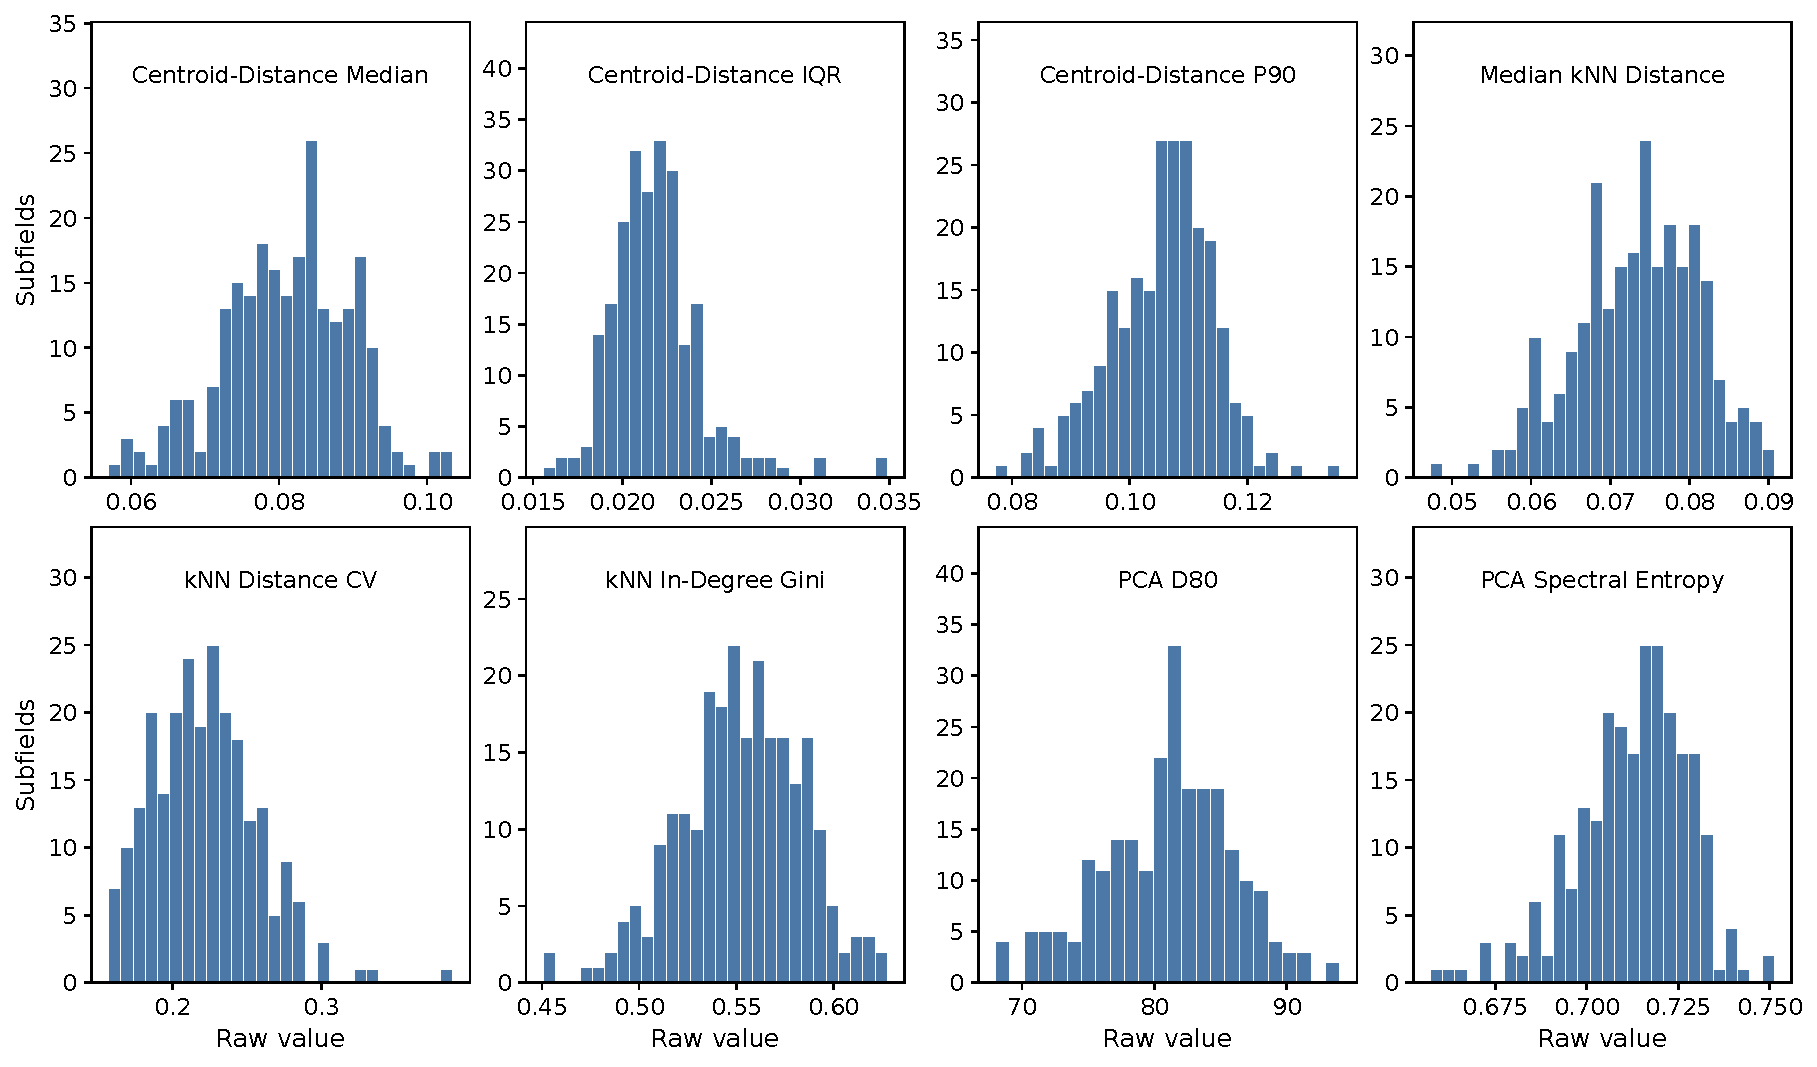
\includegraphics[height=0.72\textheight]{fig_04_structural_metric_raw_distributions.pdf}
	\end{center}

	\fignote{Several metrics are skewed or partly discrete; this motivates robust median/IQR scaling instead of z-scores.}
\end{frame}

%------------------------------------------------

\begin{frame}
	\frametitle{Backup: metric families are related but not redundant}

	\begin{columns}[c]
		\begin{column}{0.55\textwidth}
			\centering
			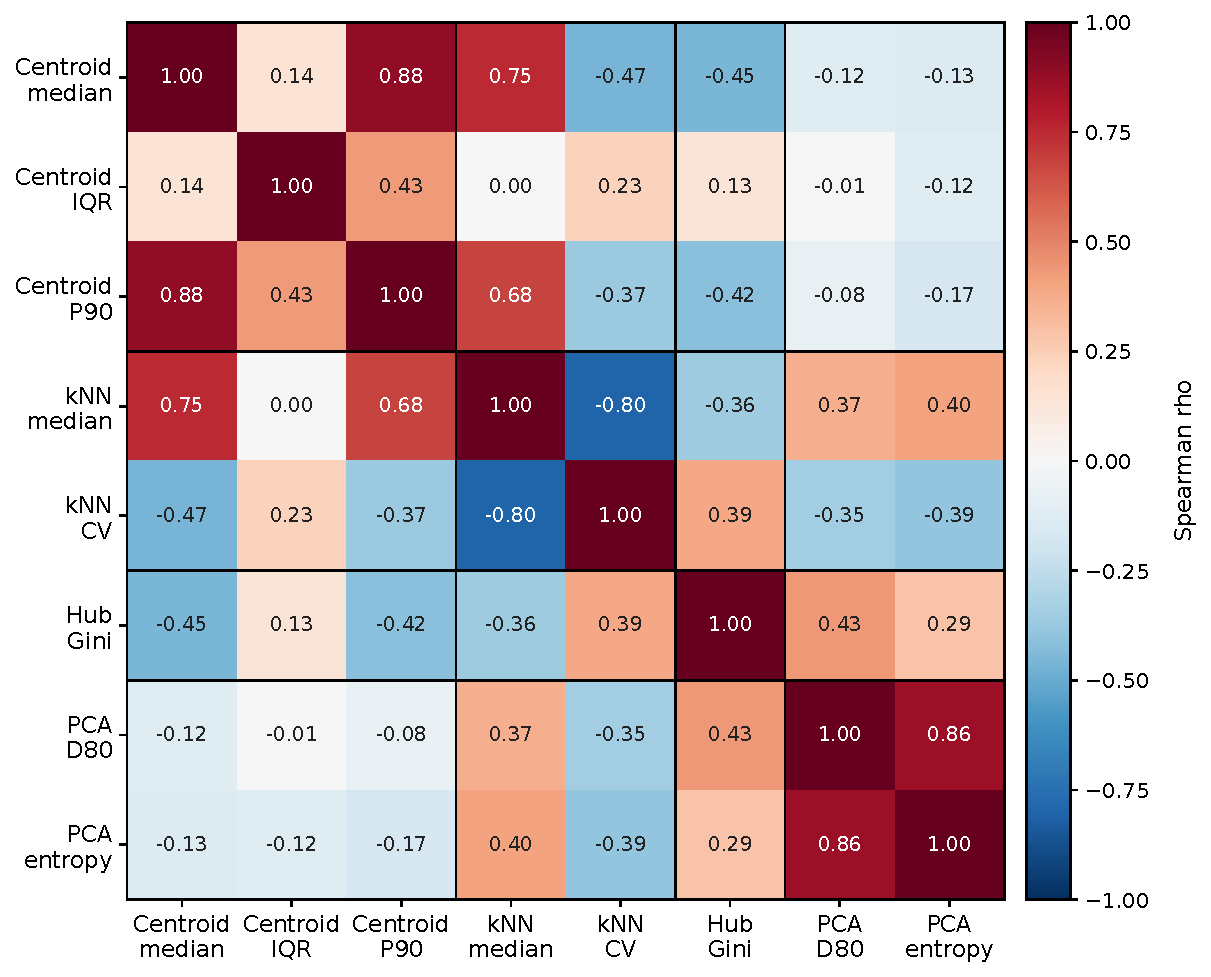
\includegraphics[height=0.80\textheight]{fig_04_structural_metric_spearman_correlation.pdf}
		\end{column}
		\begin{column}{0.43\textwidth}
			\begin{itemize}
				\setlength{\itemsep}{0.6em}
				\item Centroid median and P90: $\rho = 0.883$ (both radial spread).
				\item PCA $D_{80}$ and entropy: $\rho = 0.856$ (both spectral).
				\item kNN median and kNN CV: $\rho = -0.798$ (closer neighborhoods pack less evenly).
				\item Cross-family correlations are weaker, supporting four separate families.
			\end{itemize}
		\end{column}
	\end{columns}
\end{frame}

%------------------------------------------------

\begin{frame}
	\frametitle{Backup: full distributions by domain}

	\begin{center}
		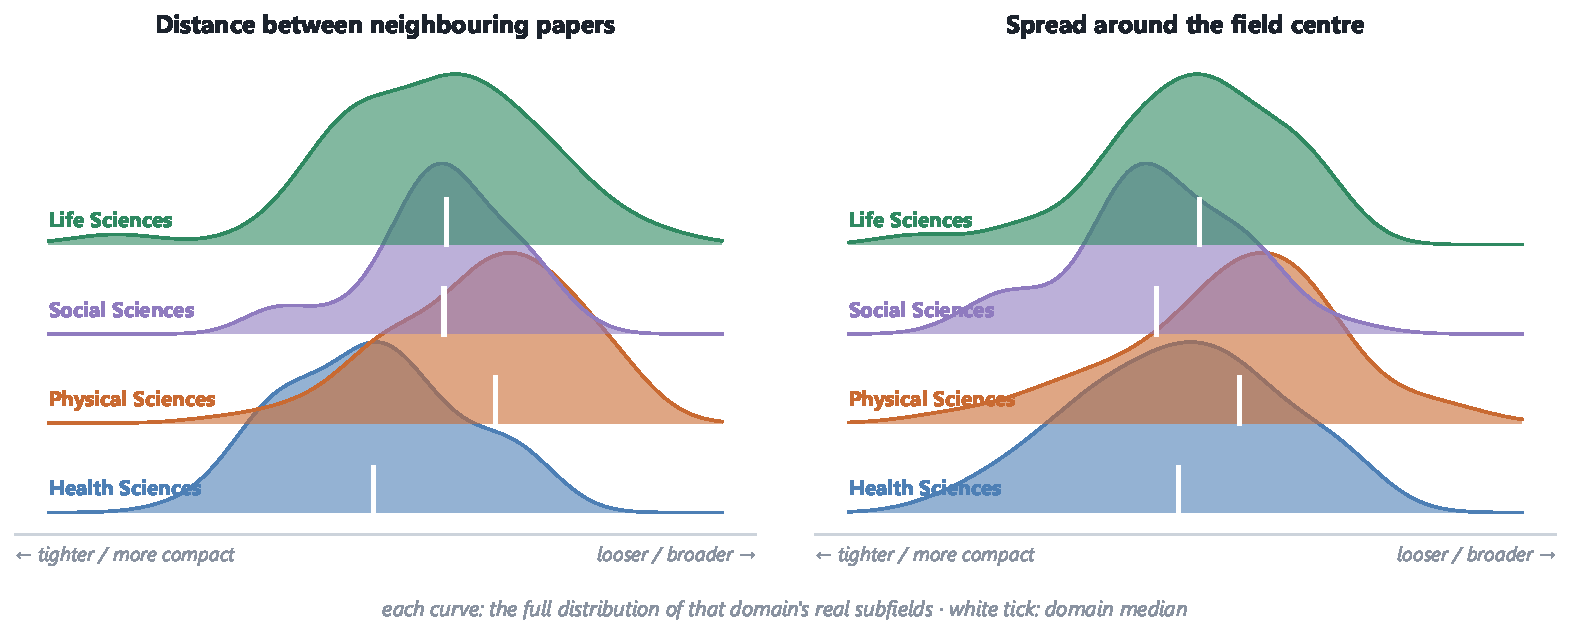
\includegraphics[width=0.95\linewidth]{def_opt_ridges.pdf}
	\end{center}
\end{frame}

%------------------------------------------------

\begin{frame}
	\frametitle{Backup: subfield profile space (PCA of standardized profiles)}

	\begin{center}
		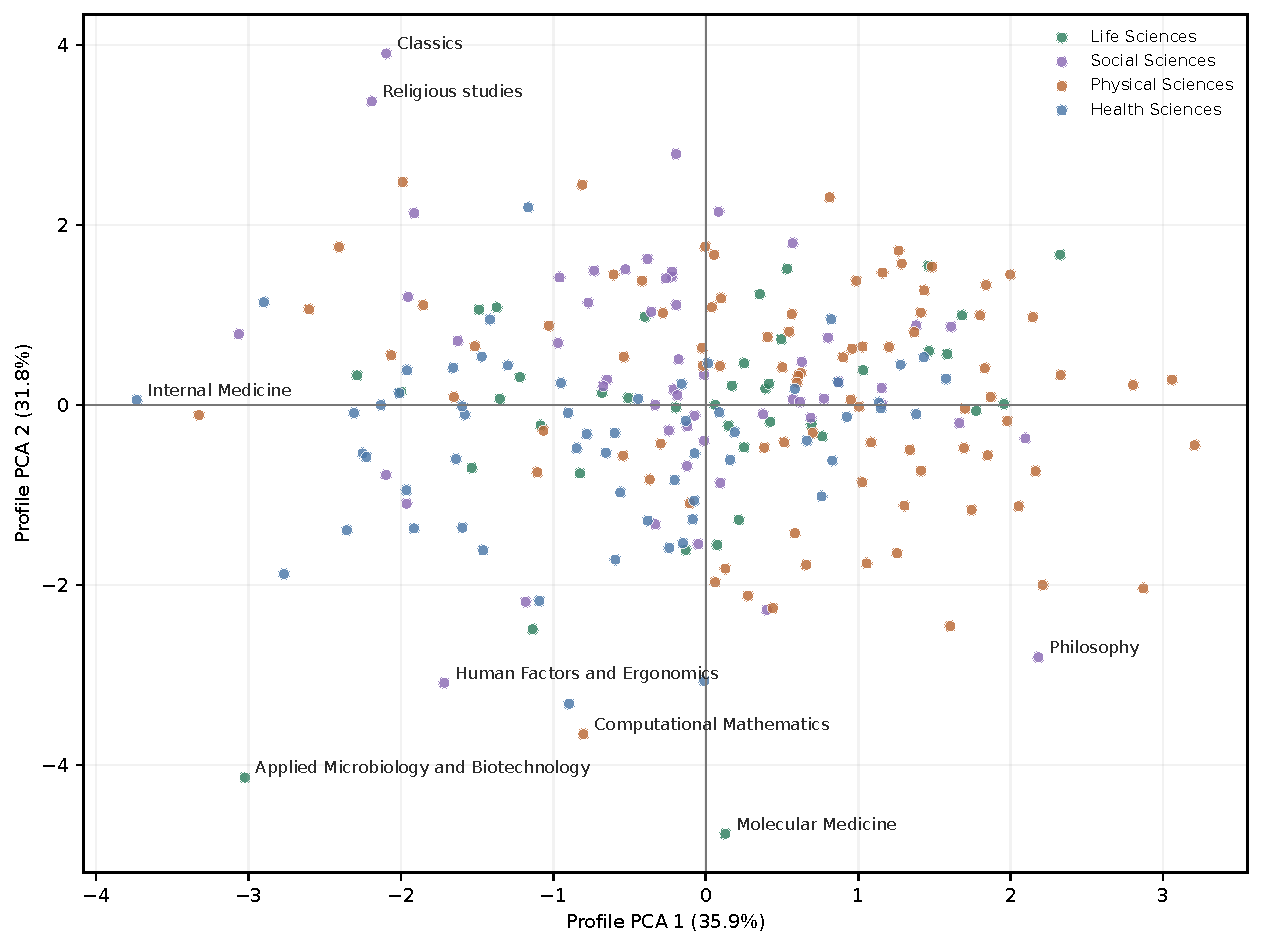
\includegraphics[height=0.72\textheight]{fig_04_metric_profile_pca_map.pdf}
	\end{center}

	\fignote{First two axes explain 35.9\% and 31.8\% of profile variance. Domains overlap near the centre; the informative cases are subfields at the edges.}
\end{frame}

%------------------------------------------------

\begin{frame}
	\frametitle{Backup: two structural opposites, metric by metric}

	\begin{center}
		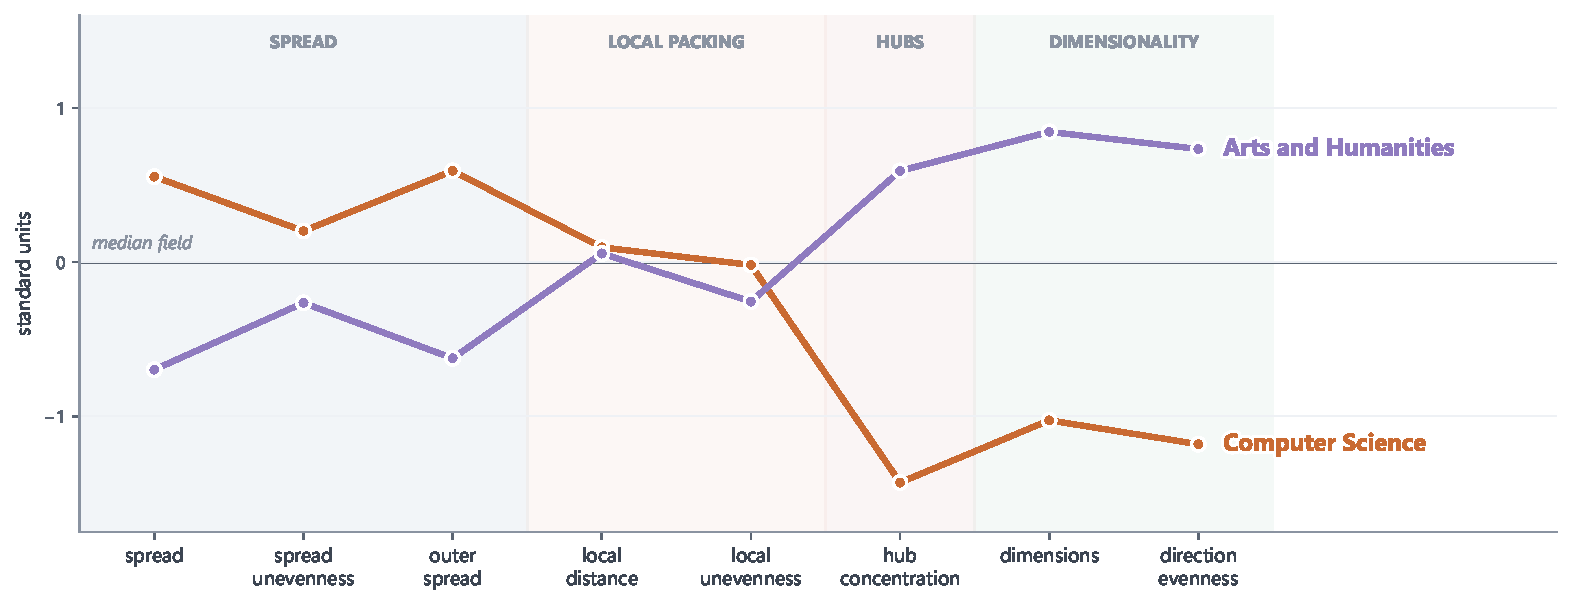
\includegraphics[width=0.92\linewidth]{def_mirror_profiles.pdf}
	\end{center}

	\fignote{Real standardized field profiles. Computer Science is broad but hub-free and low-dimensional; Arts and Humanities is its mirror image.}
\end{frame}

%------------------------------------------------

\begin{frame}
	\frametitle{Backup: all 325 field pairs by shape difference}

	\begin{center}
		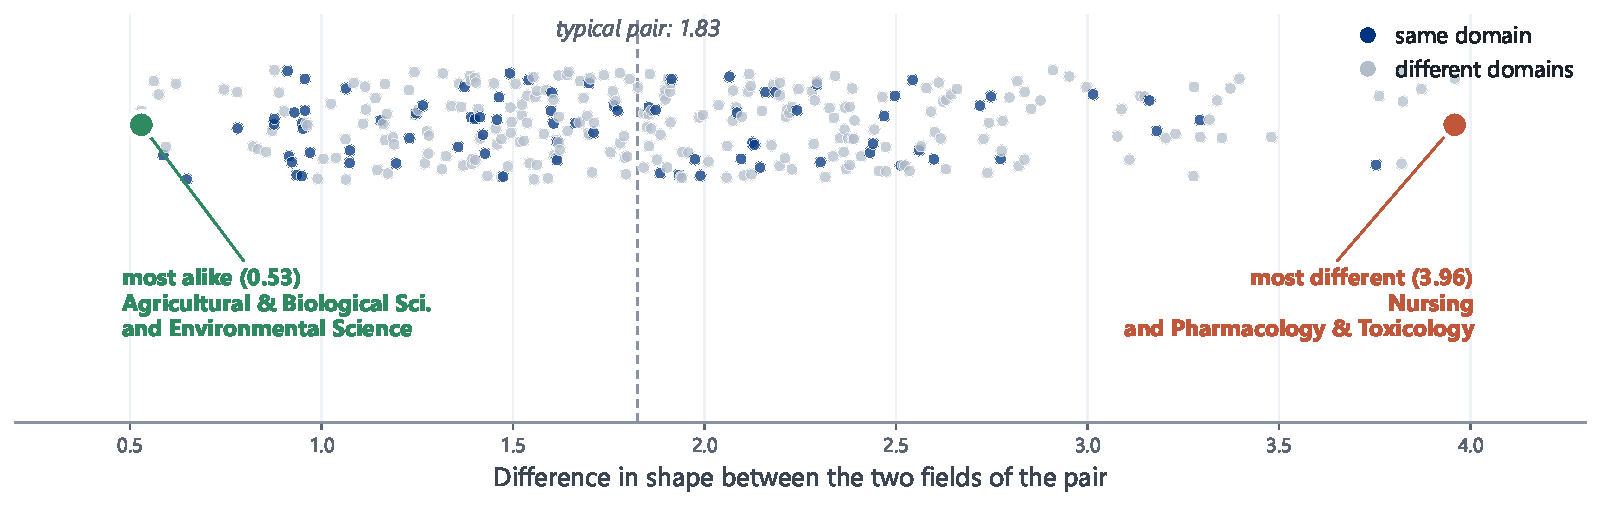
\includegraphics[width=0.94\linewidth]{def_field_similarity.pdf}
	\end{center}

	\fignote{Median pair difference 1.83; the closest pairs are mostly cross-domain.}
\end{frame}

%------------------------------------------------

\begin{frame}
	\frametitle{Backup: the kind of claims this thesis makes}

	\begin{block}{Descriptive and comparative by design}
		How fields differ and change under one fixed corpus, taxonomy, model, and metric set. Not why, not how well, not how much they are worth.
	\end{block}

	\medskip

	\begin{itemize}
		\setlength{\itemsep}{0.6em}
		\item Under that fixed design, the 241 subfields are the \textbf{whole population} of analysis units, not a sample from one; classical significance tests would answer a different question.
		\item Where variability does matter, it is quantified: the dynamic typology holds a \textbf{subsample bootstrap ARI of 0.725}.
		\item Robust median/IQR scaling keeps any single extreme subfield from driving a comparison.
		\item No claims about quality, impact, value, or causal mechanisms.
	\end{itemize}
\end{frame}

%------------------------------------------------

\begin{frame}
	\frametitle{Backup: the four trajectory patterns}

	\begin{center}
		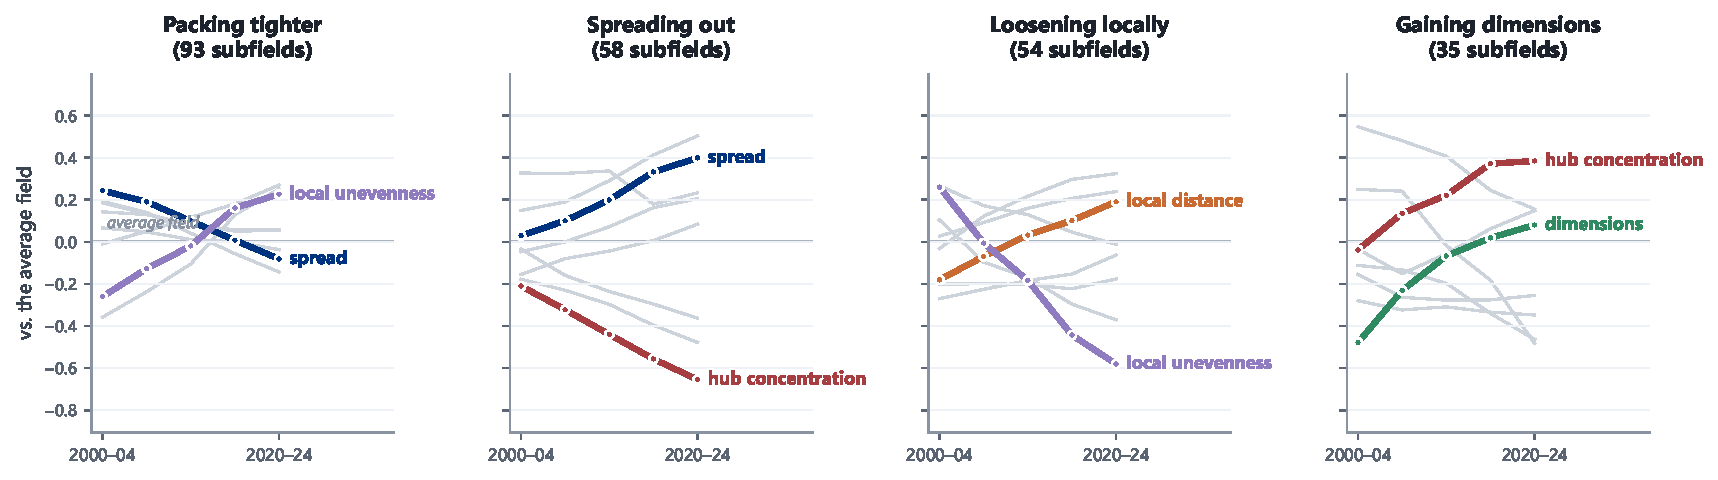
\includegraphics[width=0.96\linewidth]{def_trajectory_patterns.pdf}
	\end{center}

	\medskip
	\centering
	\small Cluster quality: silhouette 0.396 and subsample ARI 0.725 ($k=4$), versus silhouette 0.174 for clustering on static profiles ($k=5$).
\end{frame}

%------------------------------------------------

\begin{frame}
	\frametitle{Backup: domain-level temporal trajectories, all eight metrics}

	\begin{center}
		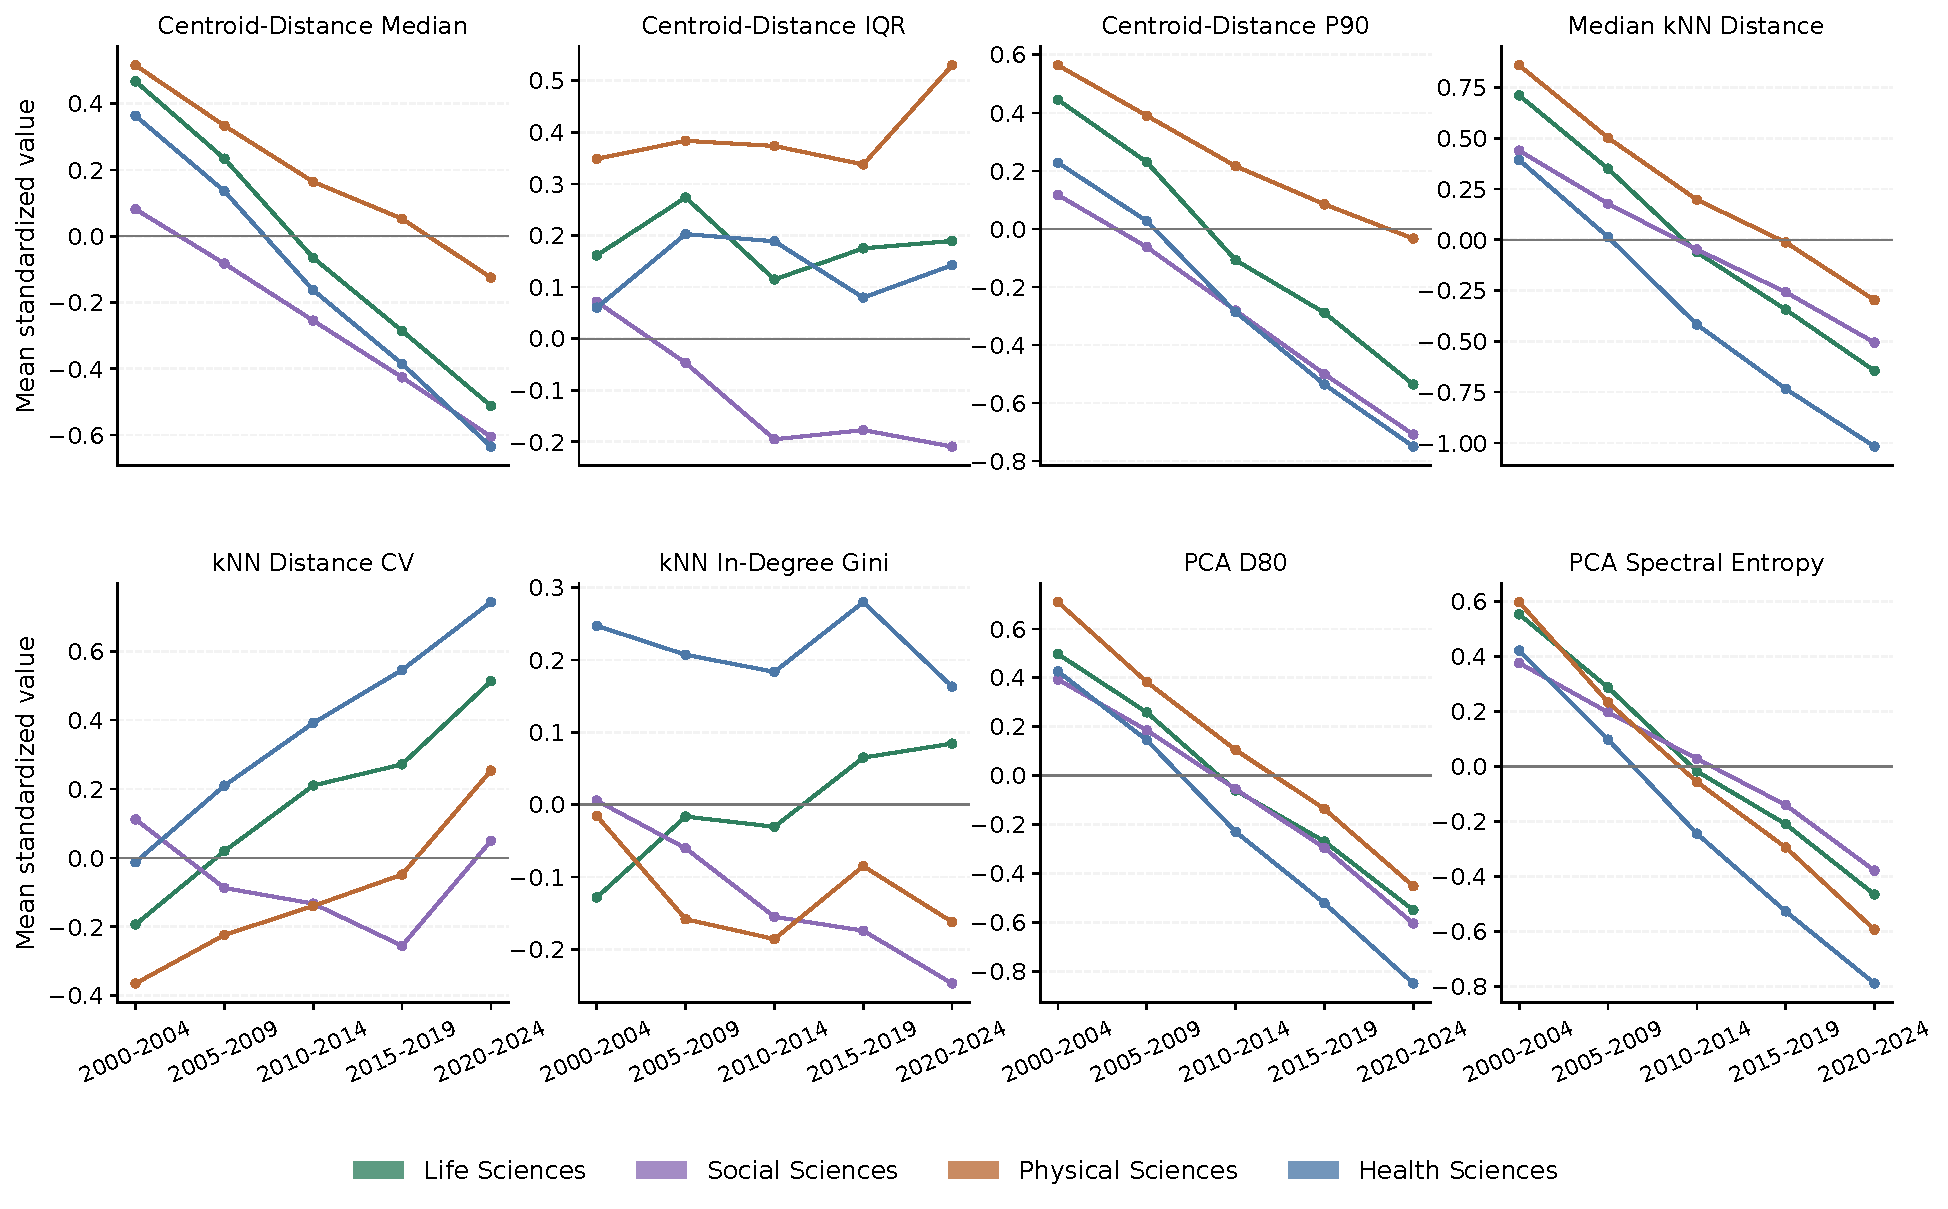
\includegraphics[height=0.80\textheight]{fig_05_domain_temporal_trajectories.pdf}
	\end{center}
\end{frame}

%------------------------------------------------

\begin{frame}
	\frametitle{Backup: what is happening to Computer Science}

	\begin{center}
		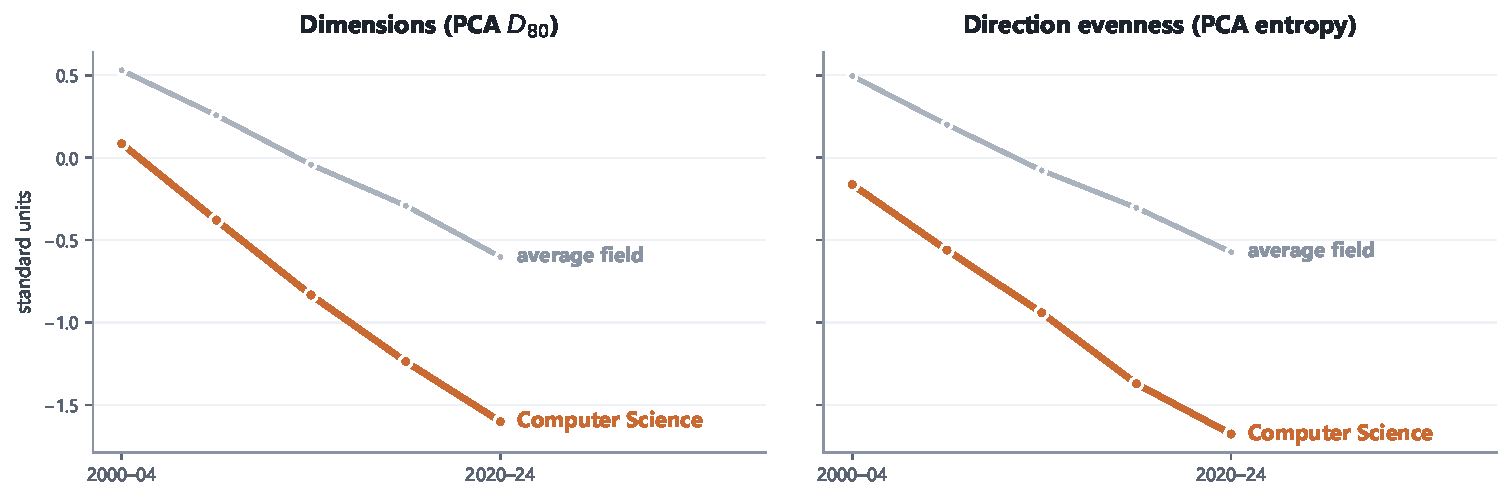
\includegraphics[width=0.95\linewidth]{def_cs_collapse.pdf}
	\end{center}

	\smallskip
	\centering
	Its variation collapses onto fewer, more dominant directions, much faster than science overall. That spectral collapse drives its nine largest divergences.
\end{frame}

%------------------------------------------------

\begin{frame}
	\frametitle{Backup: each field's nearest neighbour, and the two isolates}

	\begin{center}
		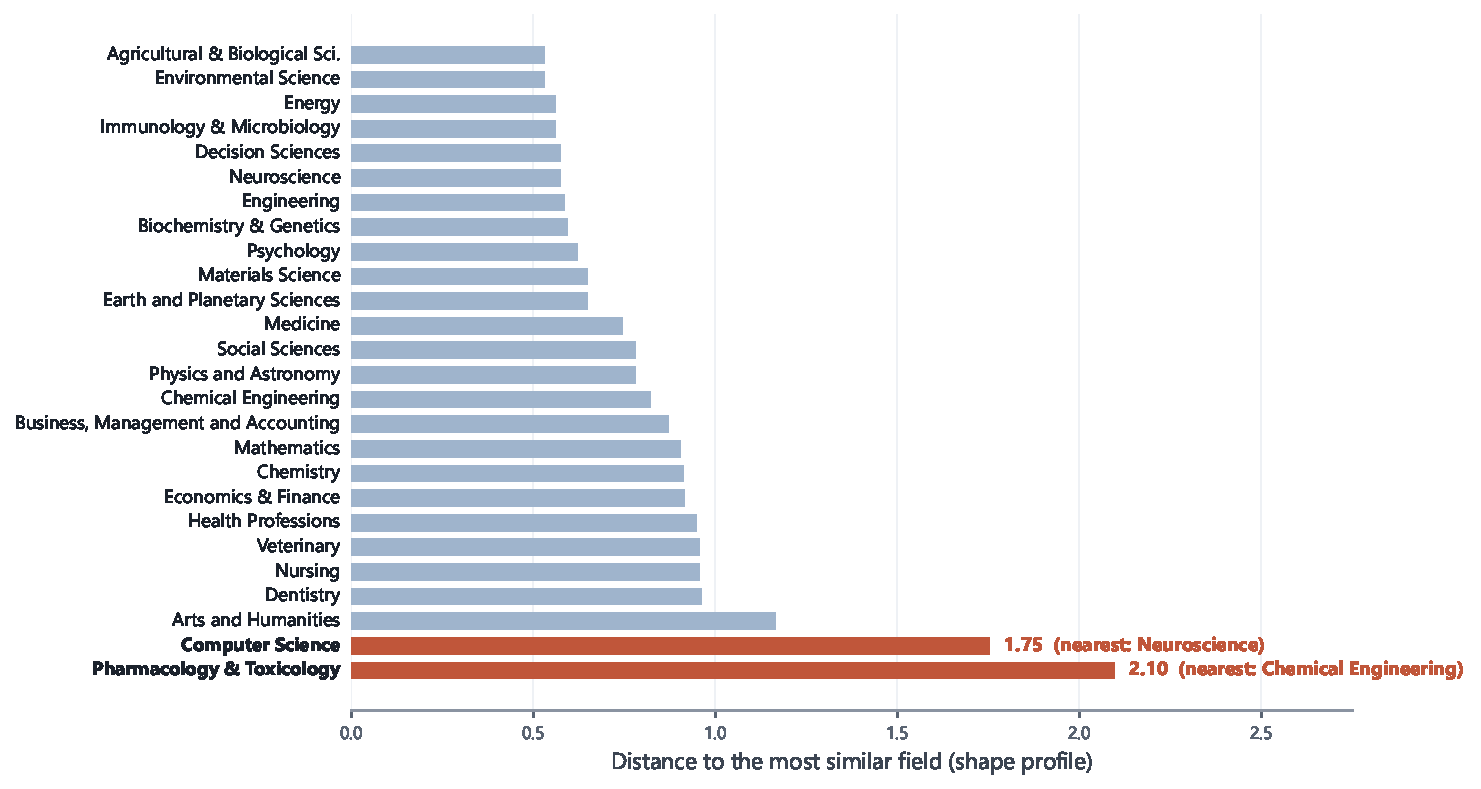
\includegraphics[height=0.80\textheight]{def_isolates.pdf}
	\end{center}
\end{frame}

%------------------------------------------------

\begin{frame}
	\frametitle{Backup: why every subfield has the same yearly cap}

	\begin{itemize}
		\setlength{\itemsep}{0.6em}
		\item kNN distances and PCA depend \textbf{mechanically} on sample size: more papers means closer neighbours and more components, regardless of any real structure.
		\item Without a cap, large fields would look dense and low-dimensional simply because they publish more.
		\item With the cap (400 papers per subfield and year, 10{,}000 over the period), every cloud is measured at a comparable $n$.
		\item Unused capacity is never moved to other years or subfields, and gaps are never imputed, so volume cannot re-enter the design.
	\end{itemize}

	\medskip

	\begin{block}{The consequence}
		Fields are compared on shape, never on publication volume.
	\end{block}
\end{frame}

%------------------------------------------------

\begin{frame}
	\frametitle{Backup: corpus validation}

	\begin{itemize}
		\setlength{\itemsep}{0.55em}
		\item Eligibility: English articles and preprints, 2000--2024, with sufficient title--abstract text.
		\item Checks passed: no duplicates, no out-of-period rows, no missing taxonomy or text fields, no disallowed types.
		\item Of 6{,}300 subfield--year cells, \textbf{5{,}493} reach the 400-work target; 807 sparse cells are coverage limits, not failures.
		\item Sparse capacity is \alert{not} reallocated and gaps are \alert{not} imputed, so volume cannot re-enter the design.
		\item Temporal matrix nearly complete: 1{,}204 of 1{,}205 subfield--window profiles (Computational Mathematics 2000--2004 excluded from first--last comparisons).
	\end{itemize}
\end{frame}

%------------------------------------------------

\begin{frame}
	\frametitle{Backup: robustness and validation agenda}

	\begin{block}{Representation}
		Rerun the identical pipeline with other scientific embedding models, full-text input, and multilingual corpora; one component swapped at a time.
	\end{block}

	\medskip

	\begin{block}{Design sensitivity}
		Sweep $k$ in the neighbour metrics; replace five-year blocks with annual and rolling windows; alternative taxonomies to the OpenAlex hierarchy.
	\end{block}

	\medskip

	\begin{block}{External validation}
		Compare morphology with evidence deliberately excluded from its construction: citation networks, funding categories, and expert review of the extreme cases (Philosophy, Computer Science, Pharmacology).
	\end{block}
\end{frame}

\backupend

%----------------------------------------------------------------------------------------

\end{document}
